\documentclass[pdflatex,sn-mathphys-num]{sn-jnl}
\usepackage{graphicx}
\usepackage{multirow}
\usepackage{amsmath,amssymb,amsfonts}
\usepackage{amsthm}
\usepackage{mathrsfs}
\usepackage[title]{appendix}
\usepackage{xcolor}
\usepackage{textcomp}
\usepackage{manyfoot}
\usepackage{booktabs}
\usepackage{algorithm}
\usepackage{algorithmicx}
\usepackage{algpseudocode}
\usepackage{listings}

\newcommand{\dgm}[0]{\mathrm{dgm}}
\newcommand{\card}[0]{\mathrm{card}}

\newtheorem{theorem}{Theorem}
\newtheorem{proposition}[theorem]{Proposition}
\newtheorem{corollary}{Corollary}
\newtheorem{lemma}{Lemma}
%\theoremstyle{thmstyletwo}
\newtheorem{example}{Example}
\newtheorem{remark}{Remark}
\newtheorem{definition}{Definition}

\newcommand{\bigzero}{\mbox{\normalfont\Large\bfseries 0}}
\newcommand{\cupdot}{\mathbin{\mathaccent\cdot\cup}}

\makeatletter
\newsavebox{\@brx}
\newcommand{\llangle}[1][]{\savebox{\@brx}{\(\m@th{#1\langle}\)}%
  \mathopen{\copy\@brx\kern-0.5\wd\@brx\usebox{\@brx}}}
\newcommand{\rrangle}[1][]{\savebox{\@brx}{\(\m@th{#1\rangle}\)}%
  \mathclose{\copy\@brx\kern-0.5\wd\@brx\usebox{\@brx}}}
  \makeatother
\newcommand\restr[2]{{% we make the whole thing an ordinary symbol
  \kern-\nulldelimiterspace % automatically resize the bar with \right
  #1 % the function
  \vphantom{\big|} % pretend it's a little taller at normal size
  \right|_{#2} % this is the delimiter
  }}

\raggedbottom

\begin{document}

\title[Spectral relaxation of the persistence rank invariant]{Spectral relaxation of the persistence rank invariant}

\author*[1]{\fnm{Matthew} \sur{Piekenbrock}}\email{piekenbrock.m@northeastern.edu}
\author[1,2]{\fnm{Jose} \sur{Perea}}\email{jose.perea@northeastern.edu}

\affil[1]{
	\orgdiv{Khoury College of Computer Sciences}, 
	\orgname{Northeastern University}
%	\orgaddress{
%%		\street{440 Huntington Avenue}, 
%		\city{Boston}, 
%%		\postcode{02115}, 
%		\state{MA}, \country{USA}
%	}
}

\affil[2]{
	\orgdiv{Department of Mathematics}, 
	\orgname{Northeastern University}
%	\orgaddress{
%%		\street{440 Huntington Avenue}, 
%		\city{Boston}, 
%%		\postcode{02115}, 
%		\state{MA}, \country{USA}
%	}
}

\abstract{
	Using a duality result between persistence diagrams and persistence measures, we introduce a framework for constructing families of continuous relaxations of the persistent rank invariant for parametrized families of persistence vector spaces indexed over the real line. Like the rank invariant, these families obey inclusion-exclusion, derive from simplicial boundary operators, and encode all the information needed to construct a persistence diagram. 
	Unlike the rank invariant, these spectrally-derived families enjoy a number of stability and continuity properties, such as smoothness and differentiability over the positive semi-definite cone. 
	Surprisingly, by leveraging a connection between stochastic Lanczos quadrature and implicit trace estimation, our proposed relaxation enables the matrix-free, iterative approximation scheme for all of the persistence invariants---Betti numbers, persistent pairs, and cycle representatives---in linear space and cubic time in the size of the filtration. 
}
\keywords{Topological Data Analysis, Persistent Homology, Matrix functions}
\pacs[MSC Classification]{	68Uxx, 55N31, 55-08}

\maketitle

\section{Introduction}\label{sec:intro}

Persistent homology~\cite{edelsbrunner2000topological} (PH) is the most widely deployed tool for data analysis and learning applications within the topological data analysis (TDA) community. 
Persistence-related pipelines often follow a common pattern: given a data set $X$ as input, construct a simplicial complex $K$ and an order-preserving function $f: K \to \mathbb{R}$ such that useful topological/geometric information may be gleaned from its persistence diagram—a multiset summary of $f$ formed by pairs $(a, b) \in \mathbb{R}^2$ exhibiting non-zero multiplicity $\mu_p^{a , b} \in \mathbb{Z}_+$ \cite{cerri2013betti}: 
\begin{align}
	\dgm_p (K, f) &= \{ (a,b) : \mu_p^{a,b} \neq 0 \} \\
	\mu_p^{a,b} &= \min_{\delta > 0} (\beta_p^{a+\delta, b-\delta} - \beta_p^{a+\delta, b+\delta}) - (\beta_p^{a-\delta, b-\delta} - \beta_p^{a-\delta, b+\delta})  \label{eq:dgm}
\end{align}
\noindent The surprising and essential quality of persistence is that these pairings exist, are unique, and are stable under additive perturbations \cite{cohen2005stability}. Whether for shape recognition \cite{chazal2009gromov}, dimensionality reduction \cite{scoccola2023fibered}, or time series analysis \cite{perea2016persistent}, persistence is the de facto connection between homology and the application frontier.

\begin{figure}\label{fig:overview}
\centering
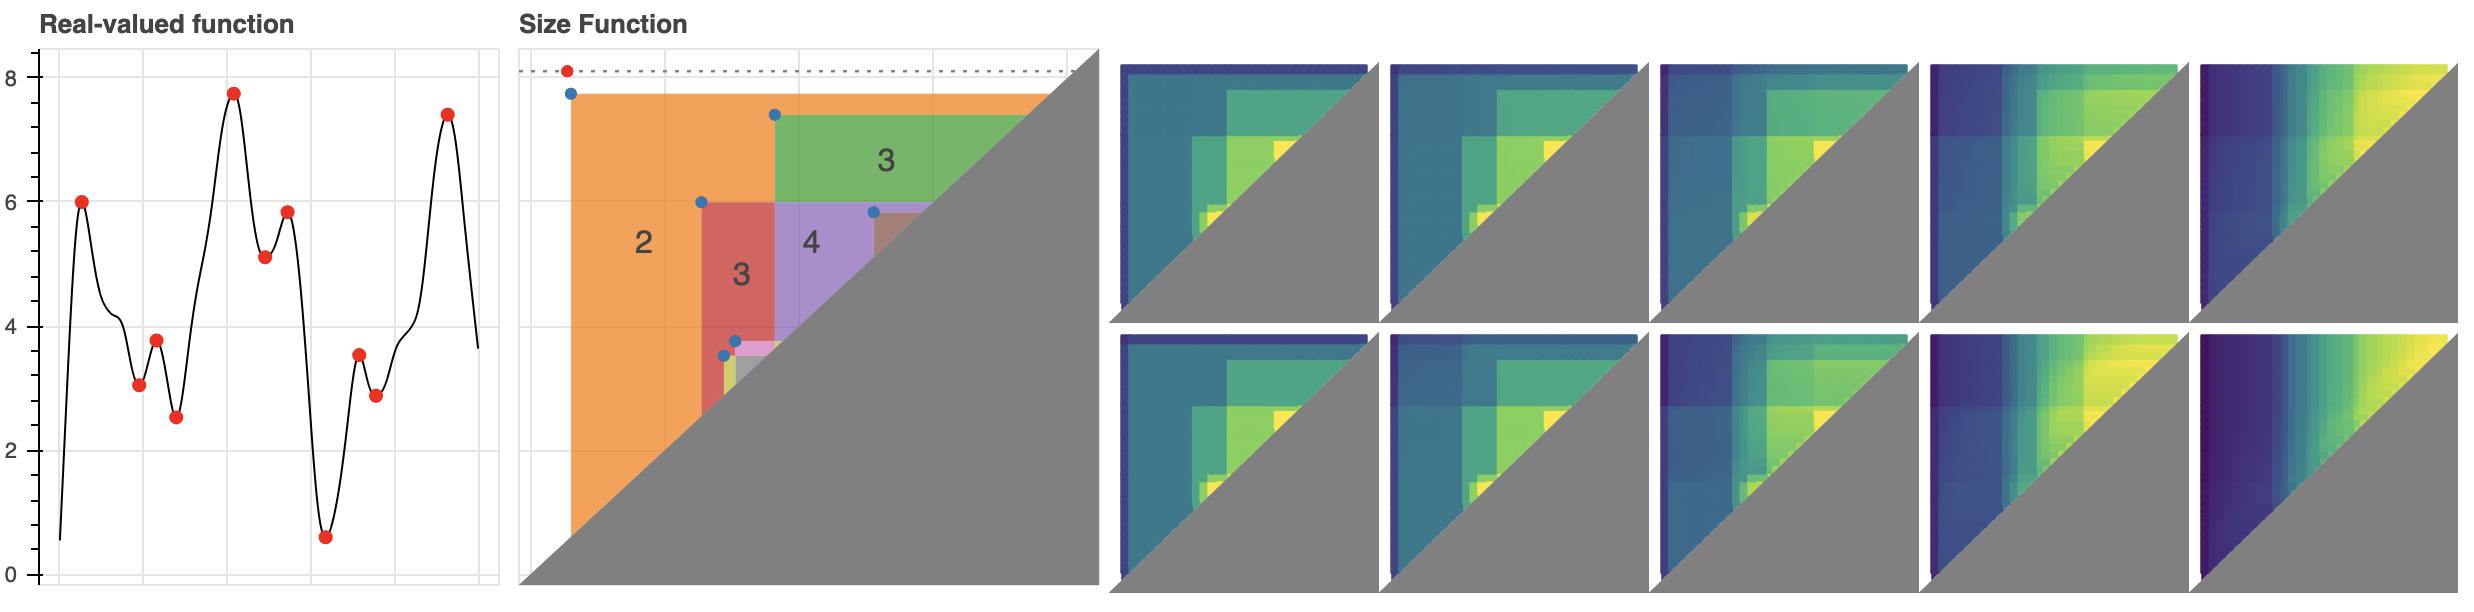
\includegraphics[width=0.95\textwidth]{../images/spectral_relax_size_func.png}	
\caption{ (left) A function $f: \mathbb{R} \to \mathbb{R}$ and its corresponding persistence diagram obtained by filtering $f$ by its sublevel sets. (right) Spectral interpolations to various Laplacian norms. }
\end{figure}

Though theoretically sound, diagrams suffer from many practical issues: they are sensitive to outliers, far from injective, and expensive---both to compute \textit{and} compare. Towards ameliorating these issues, practitioners have equipped diagrams with additional structure by way of maps to function spaces; examples include persistence images~\cite{adams2017persistence}, persistence landscapes~\cite{bubenik2015statistical}, and template functions~\cite{perea2022approximating}. Tackling the issue of injectivity, Turner et al.~\cite{turner2014persistent} propose an injective shape statistic of directional diagrams associated to a data set $X \subset \mathbb{R}^d$, sparking both an inverse theory for persistence and a mathematical foundation for metric learning. Despite the potential these extensions have in learning applications, scalability issues due to high algorithmic complexity remain. Indeed, this issue is compounded in the parameterized setting, where adaptations of the persistence computation has proven non-trivial~\cite{piekenbrock2021move}.

We seek to shift the computational paradigm on persistence while retaining its application potential: rather than following a construct-then-vectorize approach, we devise a spectral method that performs both steps, simultaneously and approximately. Our strategy is motivated both by a technical observation that suggests advantages exist for the rank invariant computation (Section~\ref{sec:betti_derivation}) and by measure-theoretic results on $\mathbb{R}$-indexed persistence modules~\cite{cerri2013betti, chazal2016structure}, which generalize Equation~\ref{eq:dgm} to rectangles $R = [a , b] \times [c , d] \subset \mathbb{R}^2$: 
\begin{equation}\label{eq:measure}
\mu_p^{R}(K, f) = \mathrm{card} (\left.\mathrm{dgm}_p(K, f)\right|_R) = 
\beta_p^{b,c} - \beta_p^{a,c} - \beta_p^{b,d} + \beta_p^{a,d}
\end{equation}
Notably, our approach not only avoids explicitly constructing diagrams, but is also \emph{matrix-free}, circumventing the reduction algorithm from~\cite{edelsbrunner2022computational} entirely. Additionally, the relaxation is computable exactly in linear space and quadratic time, requires no complicated data structures or maintenance procedures to implement, and can be iteratively $(1 \pm \epsilon)$ approximated in effectively linear time in practice for large enough $\epsilon > 0$. 
\\
\\
\noindent
\textbf{Contributions:} Our primary contribution is the introduction of several families of spectral approximations to the rank invariants—$\mu_p$ and $\beta_p$—all of which are Lipshitz continuous, and differentiable on the positive semi-definite cone ( Proposition~\ref{prop:operator_props}). Leveraging the vast spectral theory that exists for Laplacian operators ( Section~\ref{sec:laplacian_theory2}), we show these approximations are computable in $O (m)$ memory and $O (m n)$ time, where $n$ ($m$) are the number of $p$ ($p + 1$, respectively) simplices in $K$ ( Proposition~\ref{prop:spectral_rank_complexity}). Moreover, both relaxations recover their corresponding invariants when $\epsilon$ is made small enough, and both admit iterative $(1 \pm \epsilon)$-approximation schemes ( Section~\ref{sec:iterative_approx}).  

\section{Notation \& Background}\label{sec:background_notation}

A \emph{simplicial complex} \(K \subseteq \mathcal{P}(V)\) over a finite set \(V = \{ v_{1},v_{2},\ldots,v_{n}\}\) is a collection of simplices \(\{\,\sigma:\sigma \in \mathcal{P}(V)\,\}\) such that \(\tau \subseteq \sigma \in K \Rightarrow \tau \in K\). A \emph{\(p\)-simplex} \(\sigma \subseteq V\) is a set of \(p + 1\) vertices, the collection of which is denoted as \(K^{p}\). An \emph{oriented \(p\)-simplex} \( [\sigma] \) is an ordered set \( [\sigma]  = ( - 1)^{|\pi|} \left[ v_{\pi(1)},v_{\pi(2)},\ldots,v_{\pi(p + 1)} \right] \), where \(\pi\) is a permutation on \( [\, p + 1\,]  = \{\, 1,2,\ldots,p + 1\,\}\) and \(|\pi|\) the number of its inversions. The \emph{\(p\)-boundary} \(\partial_{p} [\sigma] \) of an oriented \(p\)-simplex \( [\sigma]  \in K\) is defined as the alternating sum of its oriented co-dimension 1 faces, which collectively for all \(\sigma \in K^{p}\) define the \(p\)-th \emph{boundary matrix} \(\partial_{p}\) of \(K\):
\begin{equation}
\partial_p[i, j] \triangleq 
\begin{cases}
(-1)^{s_{i j}} & \sigma_i \in \partial\left[\sigma_j\right] \\
0 & \text { otherwise }
\end{cases}, 
\quad \partial_p[\sigma] \triangleq \sum_{i=1}^{p+1}(-1)^{i-1} [v_1, \dots, v_{i-1}, v_{i+1}, \dots, v_{p+1}]
\end{equation}\label{eq:alt_sum}
\noindent
where \(s_{ij} = \operatorname{sgn} \left(  \left[ \sigma_{i} \right] ,\partial \left[ \sigma_{j} \right]  \right) \) records the orientation. Extending Equation~\ref{eq:alt_sum} to all simplices in \(\sigma \in K\) for all \(p \leq \dim(K)\) yields the \emph{full boundary matrix} \(\partial\). With a small abuse in notation, we use \(\partial_{p}\) to denote both the boundary operator and its ordered matrix representative. When it is not clear from the context, we will clarify which representation is intended.

Generalizing beyond simplices, given a field \(\mathbb{F}\), an \emph{oriented \(p\)-chain} is a formal \(\mathbb{F}\)-linear combination of oriented \(p\)-simplices of \(K\) whose boundary \(\partial_{p} [ c] \) is defined linearly in terms of its constitutive simplices. The collection of \(p\)-chains under addition yields an \(\mathbb{F}\)-vector space \(C_{p}(K)\) whose boundaries \(c \in \partial_{p} [ c'] \) satisfying \(\partial_{p} [c]  = 0\) are called \emph{cycles}. Together, the collection of \(p\)-boundaries and \(p\)-cycles forms the groups \(B_{p}(K) = \mathrm{Im}\,\partial_{p + 1}\) and \(Z_{p}(K) = \mathrm{Ker}\,\partial_{p}\), respectively. The quotient space \(H_{p}(K) = Z_{p}(K)/B_{p}(K)\) is called the \emph{\(p\)-th homology group of \(K\)} with coefficients in \(\mathbb{F}\) and its dimension \(\beta_{p}\) is the \emph{\(p\)-th Betti number} of \(K\).

A \emph{filtration} is a pair \((K,f)\) where \(f:K \rightarrow I\) is a \emph{filter function} over an index set \(I\) satisfying \(f(\tau) \leq f(\sigma)\) whenever \(\tau \subseteq \sigma\), for any \(\tau,\sigma \in K\). For every pair \((a,b) \in I \times I\) satisfying \(a \leq b\), the sequence of inclusions \(K_{a} \subseteq \ldots \subseteq K_{b}\) induce linear transformations \(h_{p}^{a,b}:H_{p}\left( K_{a} \right) \rightarrow H_{p}\left( K_{b} \right)\) at the level of homology. When \(\mathbb{F}\) is a field, this sequence of homology groups uniquely decompose \((K,f)\) into a pairing \(\left( \sigma_{a},\sigma_{b} \right)\) demarcating the evolution of homology classes~\cite{zomorodian2004computing}: \(\sigma_{a}\) marks the creation of a homology class, \(\sigma_{b}\) marks its destruction, and the difference \(\left| {a - b} \right|\) records the lifetime of the class, called its \emph{persistence}. The persistent homology groups are the images of these maps and the persistent Betti numbers are their dimensions:
\[\label{eq:pers_homology}
H_{p}^{a,b} = \begin{cases}
	H_{p}\left( K_{a} \right) & \quad a = b \\
	\operatorname{Im}\, h_{p}^{a,b} & \quad a < b
\end{cases}\:,
\quad\quad
\beta_{p}^{a,b} = \begin{cases}
	\beta_{p}\left( K_{a} \right) & \quad a = b \\
	\dim \left( H_{p}^{a,b} \right)  & \quad a < b
\end{cases}
\]
\noindent For a fixed \(p \geq 0\), the collection of persistent pairs \((a,b)\) together with unpaired simplices \((c,\infty)\) form a summary representation \(\operatorname{dgm}_{p}(K,f)\) called the \emph{\(p\)-th persistence diagram of \((K,f)\)}. Conceptually, \(\beta_{p}^{a,b}\) counts the number of persistent pairs lying inside the box \(( - \infty,a\,] \times (\, b,\infty)\)---the number of persistent homology groups born at or before \(a\) that died sometime after \(b\). When a given quantity depends on fixed parameters that are irrelevant or unknown, we use an asterisk. Thus, \(H_{p}^{\ast}(K)\) refers to any homology group of \(K\).

We will at times need to generalize the notation given thus far to the \emph{parameterized} setting. Towards this end, for some \(\mathcal{A} \subseteq \mathbb{R}^{d}\), we define an \emph{\(\mathcal{A}\)-parameterized filtration} as a pair \(\left( K,f_{\alpha} \right)\) where \(K\) is a simplicial complex and \(f:K \times \mathcal{A} \rightarrow \mathbb{R}\) an \(\mathcal{A}\)-parameterized filter function satisfying:
\begin{equation*}
f_{\alpha}(\tau) \leq f_{\alpha}(\sigma)\:\forall\:\tau \subseteq \sigma \in K\text{ and }f_{\alpha}(\sigma)\text{ is continuous in }\alpha \in \mathcal{A}\text{ for every }\sigma \in K
\end{equation*}
Intuitively, when \(\mathcal{A} = \mathbb{R}\), one can think of \(\alpha\) as a \emph{time} parameter and each \(f_{\alpha}(\sigma)\) as tracing a curve in \(\mathbb{R}^{2}\) parameterized by \(\alpha\). Examples of parameterized filtrations include:
\begin{itemize}
\item
  (Constant filtration) For a filter \(f:K \rightarrow \mathbb{R}\), note \(\left( K,f_{\alpha} \right)\) generalizes the ``static'' notion of a filtration \((K,f)\) in the sense one may declare \(f_{\alpha}(\sigma) = f(\sigma)\) for all \(\alpha \in \mathcal{A}\) and all \(\sigma \in K\).
\item
  (Dynamic Metric Spaces) For a set \(X\), let \(\gamma_{X} =  \left( X,d_{X} ( \cdot )  \right) \) denote a dynamic metric space~\cite{kim2021spatiotemporal}, where \(d_{X} ( \cdot ) :\mathbb{R} \times X \times X\) denotes a time-varying metric. For any fixed \(K \subset \mathcal{P}(X)\), the pair \(\left( K,f_{\alpha} \right)\) obtained by setting \(f_{\alpha}(\sigma) = \max\limits_{x,x' \in \sigma}d_{X}(\alpha)(x,x')\) recovers the notion of a \emph{time-varying Rips filtration}.
\item
  (Interpolating filtrations) For \(f,g:K \rightarrow \mathbb{R}\) filters over \(K\), a natural family of filtrations \(\left( K,h_{\alpha} \right)\) is obtained by choosing a homotopy \(h:\mathbb{R} \times [ 0,1] \rightarrow \mathbb{R}\) satisfying \(h_{0} = f\) and \(h_{1} = g\).
\end{itemize}

\begin{itemize}
\item
  (Fibered barcode) For a 2-d persistence module \(M\), a common invariant of interest is the \emph{fibered barcode}, which is the collection of barcodes of \(1\)-d affine slices of \(M\). These affine slices are themselves restrictions of a bifiltration parameterized by a 2-parameter family of lines homeomorphic to \([ 0,1] \times \mathbb{R}\)~\cite{lesnick2015interactive}.
\end{itemize}

\subsection{Technical background}\label{sec:betti_derivation}
The following results summarize some technical observations motivating this effort, which will be used in several proofs. Though these observations serve as background material, they contextualize our non-traditional computation of the rank invariant ( Corollary~\ref{cor::rank_reduction}) and serve as the motivation for this work.

Among the most widely known results for persistence is the structure theorem~\cite{zomorodian2004computing}, which shows 1-parameter persistence modules decompose in an \emph{essentially unique} way. Computationally, the corresponding Pairing Uniqueness Lemma~\cite{cohen2006vines} asserts that if \(R = \partial V\) decomposes the boundary matrix \(\partial \in \mathbb{F}^{N \times N}\) to a \emph{reduced} matrix \(R \in \mathbb{F}^{N \times N}\) using left-to-right column operations, then:
\begin{equation}
	R [i,j]  \neq 0 \Leftrightarrow \operatorname{rank} \left( \partial^{i,j} \right)  - \operatorname{rank} \left( \partial^{i\mathtt{+}1,j} \right)  + \operatorname{rank} \left( \partial^{i\mathtt{+}1,j\mathrm{-}1} \right)  - \operatorname{rank} \left( \partial^{i,j\mathrm{-}1} \right)  \neq 0
\end{equation}\label{eq:uniq_pivot}
\noindent
where \(\partial^{i,j}\) denotes the lower-left submatrix defined by the first \(j\) columns and the last \(m - i + 1\) rows (rows \(i\) through \(m\), inclusive). Thus, the existence of non-zero ``pivot'' entries in \(R\) may be inferred entirely from the ranks of certain submatrices of \(\partial\). Part of the validity of Equation~\ref{eq:uniq_pivot} can be attributed to the following Lemma:
\begin{lemma}\label{lemma:rank}
		Given filtration $(K , f)$ of size $N = \lvert K \rvert$, let $R = \partial V$ denote the decomposition of the filtered boundary matrix $\partial \in \mathbb{F}^{N \times N}$. Then, for any pair $(i , j)$ satisfying $1 \leq i < j \leq N$, we have: 
		\begin{equation}\label{eq:lower_left_rank}
			\mathrm{rank} (R^{i, j}) = \mathrm{rank}(\partial^{i , j}) 
		\end{equation}
		Equivalently, all lower-left submatrices of $\partial$ have the same rank as their corresponding submatrices in $R$.
\end{lemma}
\noindent An explicit proof of both of these facts can be found in \cite{dey2022computational}, though the latter was also noted in passing by Edelsbrunner \cite{edelsbrunner2000topological}. Though typically used to prove the correctness of the reduction algorithm, the implications of these two observations are are quite general, as recently noted by \cite{bauer2022keeping}:

\begin{corollary}[Bauer et al.~\cite{bauer2022keeping}]
	Any matrix reduction algorithm which preserves the ranks of the submatrices $\partial^{i , j} (K , f)$ for all $i, j \in [N]$ satisfying $1 \leq i < j \leq N$ is a valid persistence algorithm.
\end{corollary}\label{cor:valid_pers}
\noindent Indeed, though \(R\) is not unique, its non-zero pivots are, and these pivots \emph{define} the persistence diagram. Moreover, due to Equation~\ref{eq:lower_left_rank}, both \(\beta_{p}^{\ast}\) and \(\mu_{p}^{\ast}\) may be written as a sum of ranks of submatrices of \(\partial_{p}\) and \(\partial_{p + 1}\):

\begin{corollary}
	Given a fixed $p \geq 0$, a filtration $(K , f)$ with filtration values $ \{ a_i \}_{i = 1}^N$, and a rectangle $R = [a_i , a_j] \times [a_k , a_l] \subset \Delta_+$, the persistent Betti and multiplicity functions may be written as:
	\begin{align}
	\beta_p^{a_i, a_j}(K, f) &= \mathrm{rank}(C_p (K_i)) - \mathrm{rank}(\partial_p^{1,i}) - \mathrm{rank}(\partial_{p+1}^{1,j}) - \mathrm{rank}(\partial_{p+1}^{i+1,j}) \label{eq:betti_four}\\
		\mu_p^R (K, f) &= \mathrm{rank}(\partial_{p+1}^{j+1, k}) - \mathrm{rank}(\partial_{p+1}^{i+1, k}) - \mathrm{rank}(\partial_{p+1}^{j+1, l}) + \mathrm{rank}(\partial_{p+1}^{i+1, l}) \label{eq:mu_four}
	\end{align}
\end{corollary}\label{cor:rank_reduction}
\noindent Though Equation~\ref{eq:mu_four} was pointed out by Cohen-Steiner et al. in \cite{cohen2006vines} and exploited computationally by Chen \& Kerber in \cite{chen2011output}, to the authors knowledge the only explicit derivation and proof of Equation~\ref{eq:betti_four} is given by Dey \& Wang \cite{dey2022computational}. For completeness, we give our own detailed proof of Corollary~\ref{cor:rank_reduction} in Section~\ref{sec:proofs}. In practice, neither expressions seem used in any commonly used persistence software.

Two important properties of the expressions from Corollary~\ref{cor:rank_reduction} are: (1) they are comprised strictly of \emph{rank} computations, and (2) all terms involve \emph{unfactored} boundary matrices. Coupled with measure-theoretic perspectives on persistence \cite{chazal2016structure}, the former suggests variational perspectives of the rank function might yield interesting spectral relaxations of the expressions from Corollary~\ref{cor:rank_reduction} useful for e.g. optimization purposes. Both the latter property with Corollary~\ref{cor:valid_pers} suggests a potentially new means of computing persistence information \emph{without} matrix reduction. Moreover, combining these observations suggests advances made in other areas of applied mathematics may be readily exploited, such as the rich theory of matrix functions \cite{bhatia2013matrix}, the tools developed as part of ``The Laplacian Paradigm'' \cite{teng2010laplacian}, or the recent connections between rank and trace estimation \cite{ubaru2016fast}. The rest of the paper is dedicated to exploring these connections and their implications.

\subsection{Spectral relaxation and its implications}\label{sec:spectral_sec}

Before introducing our proposed relaxation, it is instructive to examine the how traditional expressions of the persistent rank invariants compare to those from Corollary~\ref{cor:rank_reduction}. Given a filtration \((K,f)\) of size \(N = |K|\) with \(f:K \rightarrow I\) defined over some index set \(I\), its \(p\)-th persistent Betti number \(\beta_{p}^{a,b}\) at index \((a,b) \in I \times I\), is defined as follows:
\begin{align*}
\beta_{p}^{a,b} & = \dim(Z_{p}\left( K_{a} \right)\:/\: B_{p}\left( K_{b} \right)) \\
 & = \dim(Z_{p}\left( K_{a} \right)\:/\:\left( Z_{p}\left( K_{a} \right) \cap B_{p}\left( K_{b} \right) \right)) \\
 & = \dim(Z_{p}\left( K_{a} \right)) - \dim(Z_{p}\left( K_{a} \right) \cap B_{p}\left( K_{b} \right))
\end{align*}\label{eq:pbn}
\noindent
Computationally, observe that Equation~\ref{eq:pbn} reduces to one nullity computation and one subspace intersection computation. While the former is easy to re-cast as a spectral computation, computing the latter typically requires obtaining bases via matrix decomposition. Constructing these bases explicitly using conventional \cite{bhatia2013matrix} or persistence-based \cite{zomorodian2004computing, memoli2022persistent} algorithms effectively\footnote{An alternative means to perform matrix reduction is through the PLU factorization (see \cite{dey2022computational}, section 5.1.1), which takes \(O\left( n^{\omega} \right)\) time where \(\omega \in [ 2,2.373)\) is the matrix-multiplication constant. However, this approach exploits neither the structure of the boundary matrix nor properties of persistence to accelerate the computation and is not used in practice.} requires \(\Omega \left( N^{3} \right) \) time and \(\Omega \left( N^{2} \right) \) space. As the persistence algorithm also exhibits \(O \left( N^{3} \right) \) time complexity and completely characterizes \(\beta_{p}^{a,b}\) over \emph{all} values \((a,b) \in I \times I\), there is little incentive to compute \(\beta_{p}^{a,b}\) with such direct methods (and indeed, they are largely unused). Because of this, we will focus on expressions Equation~\ref{eq:betti_four} and Equation~\ref{eq:mu_four} throughout the rest of the paper.

\subsubsection{Parameterized boundary operators}\label{sec:param_boundary}

In typical dynamic persistence settings (e.g. \cite{cohen2006vines}), a decomposition \(R = \partial V\) of the boundary matrix \(\partial\) must be permuted and modified frequently to maintain a simplexwise order respecting \(f_{\alpha}\). In contrast, the rank function is its permutation invariance: for any \(X \in \mathbb{R}^{n \times n}\) and permutation \(P\) we have: 
\[\operatorname{rank}(X) = \operatorname{rank} \left( P^{T}XP \right) \] 
This suggests persistent rank computations like those from Corollary~\ref{cor:rank_reduction} need not maintain this ordering---as long as the constitutive boundary matrices the same non-zero pattern as their filtered counterparts, their ranks will be identical. In what follows, we demonstrate how exploiting this permutation invariance significantly simplifies the practical use of Equation~\ref{eq:betti_four} and Equation~\ref{eq:mu_four} in \emph{parameterized} settings.

Let \(\left( K,f_{\alpha} \right)\) denote parameterized family of filtrations of a simplicial complex of size \(\left| K^{p} \right| = n\). Fix an arbitrary linear extension \( (K, \preceq ) \) of the face poset of \(K\). Define the \(\mathcal{A}\)-\emph{parameterized} \emph{boundary operator} \({\hat{\partial}}_{p}(\alpha) \in \mathbb{R}^{n \times n}\) of \(\left( K,f_{\alpha} \right)\) as the \(n \times n\) matrix ordered by \(\preceq\) for all \(\alpha \in \mathcal{A}\) whose entries \((k,l)\) satisfy:
\[\partial_{p}(\alpha) [ k,l]  = \begin{cases} \label{eq:param_boundary_matrix}
s_{kl} \cdot f_{\alpha}\left( \sigma_{k} \right) \cdot f_{\alpha}\left( \sigma_{l} \right) & \quad\text{if }\sigma_{k} \in \partial_{p}\left( \sigma_{l} \right) \\
0 & \quad\text{otherwise}
\end{cases} \]
\noindent where \(s_{kl} = \operatorname{sgn} \left(  \left[ \sigma_{k} \right] ,\partial \left[ \sigma_{l} \right]  \right) \) is the sign of the oriented face \( \left[ \sigma_{k} \right] \) in \(\partial \left[ \sigma_{l} \right] \). Observe that Equation~\ref{eq:param_boundary_matrix} may be decoupled into a product of diagonal matrices \(D_{\ast}\left( f_{\alpha} \right)\):
\begin{equation}\label{eq:decouple}
	\partial_{p}(\alpha) \triangleq D_{p}\left( f_{\alpha} \right) \cdot \partial_{p} \left( K_{\preceq} \right)  \cdot D_{p + 1}\left( f_{\alpha} \right)
\end{equation}
where \(D_{p}\left( f_{\alpha} \right)\) and \(D_{p + 1}\left( f_{\alpha} \right)\) are diagonal matrices whose non-zero entries are ordered by restrictions of \(f_{\alpha}\) to \(K_{\preceq}^{p}\) and \(K_{\preceq}^{p + 1}\), respectively. Clearly, \(\operatorname{rank}\left( \partial_{p}(\alpha) \right) = \operatorname{rank} \left( \partial_{p} \left( K_{\preceq} \right)  \right) \) when the diagonal entries of \(D_{p}\) and \(D_{p + 1}\) are strictly positive. Moreover, observe we may restrict to those ``lower left'' matrices from Lemma~\ref{lemma:rank} via post-composing step functions $\overline{S}_{a}(x) = \mathbf{1}_{x > a}$ and \(S_{b}(x) = \mathbf{1}_{x \leq b}(x)\) to \(D_{p}\) and \(D_{p + 1}\), respectively:
\[ \label{eq:rank_equiv_param}
{\hat{\partial}}_{p}^{a,b}(\alpha) \triangleq D_{p}\left( {\overline{S}}_{a} \circ f_{\alpha} \right) \cdot \partial_{p} \left( K_{\preceq} \right)  \cdot D_{p + 1}\left( S_{b} \circ f_{\alpha} \right)
\]
\noindent Though these step functions are discontinuous at their chosen thresholds \(a\) and \(b\), we may retain the element-wise continuity of Equation~\ref{eq:decouple} by exchanging them with clamped \emph{smoothstep} functions \(\mathcal{S}:\mathbb{R} \rightarrow  [ 0,1] \) that interpolate the discontinuous step portion of \(S\) along a fixed interval \((a,a + \omega)\), for some \(\omega > 0\) (see Figure~\ref{fig:smoothstep}).

The observations above collectively motivate our first relaxation. Without loss in generality, assume the orientation of the simplices \( (K, \preceq ) \) is induced by the order on the vertex set \(V\). To simplify the notation, we write \(A^{x} = A^{\ast ,x}\) to denote the submatrix including all rows of \(A\) and all columns of \(A\) up to \(x\).

\begin{proposition}\label{prop:mu_betti_1}
	Given $(K , f_\alpha)$, any rectangle $R = ([a , b] \times [c , d]) \subset \Delta_+$, and a constant $\delta > 0$ satisfying $a + \delta < b - \delta$ from Equation~\ref{eq:measure}, the $\mathcal{A}$-parameterized invariants $\beta_p^{a , b} : \mathcal{A} \times K \to \mathbb{N}$ and $\mu_p^{R} : \mathcal{A} \times K \to \mathbb{N}$ defined by:
	\begin{equation}\label{eq:pbn_parameterized}
		\beta_p^{a, b}(\alpha) = 
%		\mathrm{rank}( D_p (S_a \circ f_\alpha)) - 
%		\mathrm{rank}(\hat{\partial}_p^{a} (\alpha)) - 
%		\mathrm{rank}(\hat{\partial}_{p+1}^{b}(\alpha)) + 
%		\mathrm{rank}(\hat{\partial}_{p+1}^{a+\delta, b}(\alpha)) 
		\mathrm{rank} \begin{bmatrix}
			D_p (S_a \circ f_\alpha) & 0 \\
			0 & \hat{\partial}_{p+1}^{a+\delta, b}(\alpha)
		\end{bmatrix}
		-
		\mathrm{rank} \begin{bmatrix}
			\hat{\partial}_p^{a} (\alpha) & 0 \\
			0 & \hat{\partial}_{p+1}^{b}(\alpha)
		\end{bmatrix}
	\end{equation}
	\begin{equation}\label{eq:mu_parameterized}
		\mu_p^R (\alpha) = 
%		\mathrm{rank}(\hat{\partial}_{p+1}^{b+\delta, c}) - 
%		\mathrm{rank}(\hat{\partial}_{p+1}^{a+\delta, c}) - 
%		\mathrm{rank}(\hat{\partial}_{p+1}^{b+\delta, d}) + 
%		\mathrm{rank}(\hat{\partial}_{p+1}^{a+\delta, d}) 
		\mathrm{rank} \begin{bmatrix}
			\hat{\partial}_{p+1}^{b+\delta, c}(\alpha) & 0 \\
			0 & \hat{\partial}_{p+1}^{a+\delta, d}(\alpha) 
		\end{bmatrix}
		-
		\mathrm{rank} \begin{bmatrix}
			\hat{\partial}_{p+1}^{a+\delta, c}(\alpha) & 0 \\
			0 & \hat{\partial}_{p+1}^{b+\delta, d}(\alpha)
		\end{bmatrix}
	\end{equation}
	yield the correct quantities $\mu_p^R (K, f_\alpha) = \mathrm{card} (\left.\mathrm{dgm}_p (f_\alpha)\right|_R)$ and $\beta_p^{a,b} = \mathrm{dim}(H_p^{a,b}(K, f_\alpha))$ for all $\alpha \in \mathcal{A}$. 
\end{proposition}
\noindent Note that in Equation~\ref{eq:rank_equiv_param}, we write \(\partial_{p} \left( K_{\preceq} \right) \) (as opposed to \(\partial_{p}(K,f)\)) to emphasize \(\partial_{p} \left( K_{\preceq} \right) \) is ordered according to a fixed linear ordering \( (K, \preceq ) \). The distinction is necessary as evaluating the boundary terms from Corollary~\ref{cor:rank_reduction} would require \(\partial\) to be explicitly filtered in the total ordering induced by \(f_{\alpha}\)---which varies in \(\mathcal{A}\)---whereas the expressions obtained by replacing the constitutive terms in Equation~\ref{eq:betti_four} and Equation~\ref{eq:mu_four} with Equation~\ref{eq:pbn_parameterized} and Equation~\ref{eq:mu_parameterized}, respectively, requires no such explicit filtering.

\begin{corollary}
Given a boundary matrix $\hat{\partial}_p(\alpha) \in \mathbb{R}^{n \times n}$ constructed at time $\alpha \in \mathbb{R}$ from a parameterized family of filtrations $(K , f_\alpha)$ with linear extension $\preceq$, the time complexity of constructing $\hat{\partial}_p(\alpha')$ for any other $\alpha' \neq \alpha$ is $O\left( \max (\lvert K^p \rvert, \lvert K^{p + 1} \rvert ) \right)$, assuming the evaluation of $f_\alpha (\tau)$ is $O (1)$ for every simplex $\tau \in K$.
\end{corollary}

\subsection{Parameterized Laplacians}\label{sec:laplacian_theory2}

For generality's sake, it is important to make the class of expressions for \(\beta_{p}^{\ast}\) and \(\mu_{p}^{\ast}\) as large as possible. Since we are only concerned with homology over \(\mathbb{R}\), we may exploit another identity of the rank function only applicable to zero characteristic fields:
\[\label{eq:rank_invariance_adjoint}
\operatorname{rank}(X) = \operatorname{rank} \left( XX^{T} \right)  = \operatorname{rank} \left( X^{T}X \right) ,\quad\text{for all }X \in \mathbb{F}^{n \times m}
\] 
\noindent In the context of boundary operators, note that \(\partial_{1}\partial_{1}^{T}\) is the well known \emph{graph Laplacian}---more generally, Equation~\ref{eq:rank_invariance_adjoint} suggests we can readily express \(\beta_{p}^{\ast}(\alpha)\) and \(\mu_{p}^{\ast}(\alpha)\) using the ranks of combinatorial \(p\)-Laplacians.\footnote{By convention, we define \(\partial_{p} = 0\) for all \(p \leq 0\).}

Following the seminal results from Horak and Jost \cite{horak2013spectra}, there are three natural ways to define \(p\)-Laplacians over a fixed simplicial complex \(K\): the \emph{up}-Laplacian \(L_{p}^{\operatorname{up}}(K)\), the \emph{down}-Laplacian \(L_{p}^{\operatorname{dn}}(K)\), and their sum, which we refer to as the \emph{combinatorial} Laplacian \(\Delta_{p}(K)\):
\[\label{eq:comb_lap}
\Delta_{p}(K) = \underset{L_{p}^{\operatorname{up}}}{\underbrace{\partial_{p + 1} \circ \partial_{p + 1}^{T}}} + \underset{L_{p}^{\operatorname{dn}}}{\underbrace{\partial_{p}^{T} \circ \partial_{p}}}
\]
\noindent All three operators \(\Delta_{p}\), \(L_{p}^{\operatorname{up}}\), and \(L_{p}^{\operatorname{dn}}\) are symmetric, positive semi-definite, and compact \cite{memoli2022persistent}---moreover, the \emph{non-zero} multisets \(\Lambda \left( L_{p}^{\operatorname{up}} \right) \) and \(\Lambda \left( L_{p + 1}^{\operatorname{dn}} \right) \) are equivalent, implying they must have identical ranks (see Theorem 2.2 and 3.1 of \cite{horak2013spectra}). Thus, for rank computations, it suffices to consider only one of them.

Let \(\left( K,f_{\alpha} \right)\) denote a parameterized family of filtrations of a simplicial complex \(K\) equipped with a fixed but arbitrary linear extension \(\preceq\) of its face poset and fixed orientations \(s(\sigma)\) inherited from the total order on the vertex set \( (V, \preceq ) \). Without loss of generality, we define the weighted \(p\) up-Laplacian \(\mathcal{L}_{p} \triangleq L_{p}^{\operatorname{up}}\) at index \((a,b)\) as follows:
\[\begin{aligned}\label{eq:laplacian_decouple}
\mathcal{L}_{p, \preceq}^{a,b}(\alpha) & \triangleq D_{p}\left( {\overline{S}}_{a} \circ f_{\alpha} \right) \cdot \partial_{p + 1} \left( K_{\preceq} \right)  \cdot D_{p + 1}\left( S_{b} \circ f_{\alpha} \right) \cdot \partial_{p + 1}^{T} \left( K_{\preceq} \right)  \cdot D_{p}\left( {\overline{S}}_{a} \circ f_{\alpha} \right)
\end{aligned}
\]
where \(D_{p}(f)\) denotes a diagonal matrix whose entries represent the application of \(f\) to the \(p\)-simplices of \(K\). As in Equation~\ref{eq:rank_equiv_param}, fixing step function \(S_{a}\) and \({\overline{S}}_{b}\) at values \(a,b \in \mathbb{R}\) yields operators whose ranks correspond to the ranks of certain ``lower-left'' submatrices of the corresponding full boundary matrix \(\partial\) of \((K,f)\). In particular, if \(R = \partial V\) is the decomposition of \(\left( K,f_{\alpha} \right)\) for some fixed choice of \(\alpha \in \mathcal{A}\), then for any pair \((a,b) \in \Delta_{+}\) there exists indices \(i = \sum_{\sigma \in K}\left( {\overline{S}}_{a} \circ f_{\alpha} \right)(\sigma)\) and \(j = \sum_{\sigma \in K}\left( S_{b} \circ f_{\alpha} \right)(\sigma)\) such that:
\[
\operatorname{rank} \left( R_{p + 1}^{i,j} \right)  
	= \operatorname{rank} \left( \partial_{p + 1}^{i,j} \right)  = \operatorname{rank} \left( {\hat{\partial}}_{p + 1}^{a,b} \right)  
	= \operatorname{rank} \left(  \left( {\hat{\partial}}_{p + 1}^{a,b} \right)  \left( {\hat{\partial}}_{p + 1}^{a,b} \right) ^{T} \right)  
	= \operatorname{rank} \left( \mathcal{L}_{p, \preceq}^{a,b} \right) 
\]
where the second last equality uses the identity \(\operatorname{rank}(X) = \operatorname{rank} \left( X^{T}X \right) \), which holds when \(X \in \mathbb{F}^{n \times m}\) has coefficients in a zero-characteristic field \(\mathbb{F}\). This confirms that we may substitute any of the parameterized boundary operators used in Proposition~\ref{prop:mu_betti_1} with weighted Laplacian operators \(\partial_{p + 1}^{\ast} \mapsto \mathcal{L}_{p}^{\ast}\) equipped with the appropriate down- and up-step functions \(S_{\ast}\) and \({\overline{S}}_{\ast}\), respectively.

It is worth noting that composing step functions \({\overline{S}}_{a},S_{b}:\mathbb{R} \rightarrow  [ 0,1] \) with \(f_{\alpha}\) is equivalent to endowing a \emph{weight function} \(w:K \rightarrow (0, + \infty)\) on a subset \(K_{a,b} \subseteq K\), in the sense described by \cite{memoli2022persistent}. In particular, if \(w_{p}\) denotes the restriction of \(w\) to \(K^{p}\), then \(w_{p}\) defines an inner product \(\langle\, \cdot , \cdot \,\rangle_{w_{p}}\) on space of \(p\)-chains \(C_{p}\left( K,\mathbb{R} \right)\) given by:
\[\label{eq:inner_product_chain}
\langle [\sigma] , [\sigma'] \rangle_{w_{p}} \triangleq \delta_{\sigma\sigma'} \cdot \left( w_{p}(\sigma) \right)^{- 1},\quad\forall\,\sigma,\sigma' \in K^{p}
\]
where \(\delta_{\sigma\sigma'} = \mathbf{1} (\sigma = \sigma') \) is the indicator function on \(\sigma\). Moreover, this inner product \(\langle [\sigma] , [\sigma'] \rangle_{w_{p}}\) on \(C_{p}\left( K,\mathbb{R} \right)\) induces an inner product:
\[ \label{eq:inner_product_cochain}
\llangle f, g \rrangle_{w} = \sum_{\sigma \in K^{p}} f\left( [\sigma] \right)g\left( [\sigma] \right)w(\sigma),\quad\text{for all } f,g \in C^{p}(K)
\]
In these sense above, Equation~\ref{eq:laplacian_decouple} is simply choosing a particular inner product on the space of \(p\)-cochains.

\begin{remark}
	One may interpret the action of sending a subset $S \subseteq K$ of $p$-simplices to $0$ as a restriction of $K$ to a sub-complex $L = K \setminus S$, which suggests e.g. Equation~\ref{eq:pbn} and Equation~\ref{eq:laplacian_decouple} could be alternatively defined using the inclusion maps $L \hookrightarrow K$ between \textit{simplicial pairs} $(L , K)$, as in~\cite{memoli2022persistent}.
\end{remark}

% === 
\section{Spectral rank relaxation}\label{sec:spectral_relax}

Under mild assumptions on \(f_{\alpha}\), the entries of the boundary operators from Equation~\ref{eq:rank_equiv_param} are continuous functions of \(\alpha\) when \(S\) is substituted appropriately with smooth step functions. In contrast, the quantities from Proposition~\ref{prop:mu_betti_1} are by definition discontinuous functions, as they are integer-valued due to the rank function. To circumvent this issue, we consider the spectral characterization of the rank function:
\[\label{eq:rank_def}
\operatorname{rank}(X) = \sum_{i = 1}^{n}\operatorname{sgn}_{+}\left( \sigma_{i}(X) \right),\quad\quad\operatorname{sgn}_{+}(x) = \begin{cases}
\: 1 & \quad\text{if }x > 0 \\
\: 0 & \quad\text{otherwise}
\end{cases}
\]
In the above, \(\{\sigma_{i}\}_{i = 1}^{n}\) are the singular values \(\Sigma = \operatorname{diag} \left( \{\sigma_{i}\}_{i = 1}^{n} \right) \) from the singular value decomposition (SVD) \(X = U\Sigma V^{T}\) of \(X \in \mathbb{R}^{n \times m}\), and \(\operatorname{sgn}_{+}:\mathbb{R} \rightarrow \{ 0,1\}\) is the one-sided sign function. As the singular values vary continuously under perturbations in \(X\) \cite{bhatia2013matrix}, it is clear the discontinuity in Equation~\ref{eq:rank_def} manifests from the one-sided sign function---thus, for the purposes of obtaining a continuous substitute for the rank function, a natural approach is to first relax the \(\operatorname{sgn}_{+}\) function.

Our approach follows the seminal work of Mangasarian et al. \cite{mangasarian1994class}. Let \(p:\mathbb{R}_{+} \rightarrow \mathbb{R}_{+}\) denote a continuous density function and \(\nu:\mathbb{R}_{+} \rightarrow \mathbb{R}_{+}\) is a continuous increasing function satisfying \(\nu(0) = 0\). One way to approximate the \(\operatorname{sgn}_{+}\) function is to integrate \(\tau\)-smoothed variations \(\hat{\delta}\) of the Dirac delta measure \(\delta\):
\[\label{eq:phi}
\phi(x,\tau) = \int_{- \infty}^{x}\hat{\delta}(z,\tau)\operatorname{dz},\quad\hat{\delta}(z,\tau) = \frac{1}{\nu(\tau)} \cdot p\left( \frac{z}{\nu(\tau)} \right),\quad\forall z \geq 0,\tau > 0
\]
In contrast to the \(\operatorname{sgn}_{+}\) function, if \(p\) is continuous on \(\mathbb{R}_{+}\) then \(\phi ( \cdot ,\tau) \) is continuously differentiable on \(\mathbb{R}_{+}\), and if \(p\) is bounded above on \(\mathbb{R}_{+}\), then \(\phi ( \cdot ,\tau) \) is globally Lipshitz continuous on \(\mathbb{R}_{+}\). Moreover, varying \(\tau \in \mathbb{R}_{+}\) in Equation~\ref{eq:phi} yields an \(\tau\)-parameterized family of continuous \(\operatorname{sgn}_{+}\) relaxations \(\phi:\mathbb{R}_{+} \times \mathbb{R}_{+ +} \rightarrow \mathbb{R}_{+}\), where \(\tau > 0\) controls the accuracy of the relaxation.

Many properties of the sign approximation from Equation~\ref{eq:phi} extend naturally to the rank function when substituted appropriately via Equation~\ref{eq:rank_def}. In particular, pairing \(X = U\Sigma V^{T}\) with a scalar-valued \(\phi\) that is continuously differentiable at every entry \(\sigma\) of \(\Sigma\) yields a corresponding \emph{Löwner operator} \(\Phi_{\tau}\) \cite{bi2013approximation}:
\[\label{eq:lowner}
\Phi_{\tau}(X) \triangleq \sum_{i = 1}^{n}\phi\left( \sigma_{i},\tau \right)u_{i}v_{i}^{T}
\]
Note that when \(X\) is positive semi-definite, Equation~\ref{eq:lowner} may be interpreted as a particular choice of \emph{matrix function} \(f(X) \triangleq Uf(\Lambda)U^{T}\) from the matrix function calculus perspective \cite{bhatia2013matrix}. Unlike general matrix functions, however, the restrictions on \(\phi\) Equation~\ref{eq:phi} grants the operators \(\Phi_{\tau}\) a variety of attractive properties related to approximation, monotonicity, and differentiability.

\begin{proposition}[Bi et al.~\cite{bi2013approximation}]\label{prop:operator_props}
	The operator $\Phi_\tau : \mathbb{R}^{n \times m} \to \mathbb{R}^{n \times m}$ defined by Equation~\ref{eq:lowner} satisfies:
	\begin{enumerate}
		\item For any $\tau \geq 0$, the Schatten-1 norm $\lVert \Phi_\tau (X) \rVert_\ast$ of $\Phi_\tau (X)$ is given by $\sum_{i = 1}^n \phi (\sigma_i, \tau)$.
		\item For any $\tau' \geq \tau$, $\lVert \Phi_{\tau'} (X) \rVert_\ast \leq \lVert \Phi_\tau (X) \rVert_\ast$ for all $X \in \mathbb{R}^{n \times m}$.
		\item For any given $X \in \mathbb{R}^{n \times m}$ with rank $r = \mathrm{rank}(X)$ and positive singular values $\Lambda (X) = \{ \sigma_1 , \sigma_2, \dots , \sigma_r \}$, we have:
		\begin{equation}
			0 \leq r - \lVert \Phi_\tau (X) \rVert_\ast \leq r \cdot (1 - \phi(\sigma_r, \tau))
		\end{equation} 
		Moreover, if $\tau$ satisfies $0 < \tau \leq \sigma_r / r$, then $r - \lVert \Phi_\tau (X) \rVert$ is bounded above by a constant $c_\phi(r) \geq 0$.
		\item $\lVert (\Phi_\tau (X) \rVert_\ast$ is globally Lipshitz continuous and semismooth\footnote{Here, "semismooth" refers to the existence certain directional derivatives as $\tau \to 0^+$, see~\cite{bhatia2013matrix, bi2013approximation}.} on $\mathbb{R}^{n \times m}$.
	\end{enumerate}
\end{proposition}

\begin{figure}\label{fig:smoothstep}
	\centering
	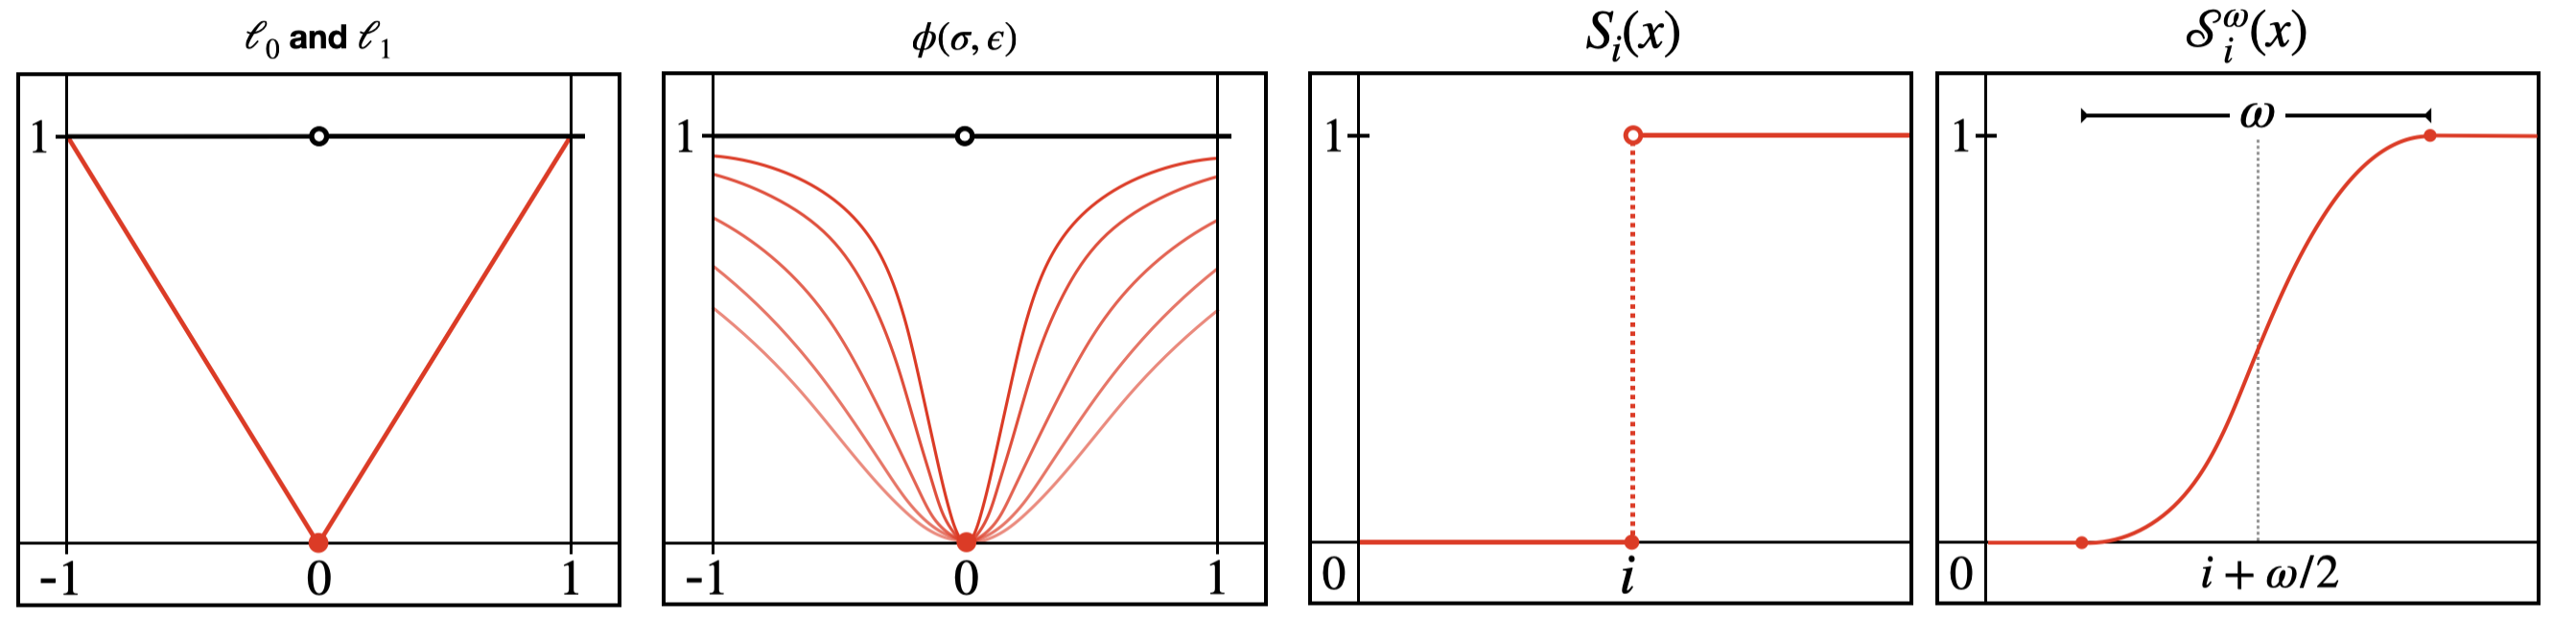
\includegraphics[width=1\linewidth,keepaspectratio]{../images/cont_relax.png}
	\caption{From left to right—the $\ell_1$ (red) norm and $\ell_0$ (black) pseudo-norm are shown on the interval $([- 1 , 1])$; the relaxation $\phi (\cdot, \tau)$ from Equation~\ref{eq:tikhonov_sf} at various values of $\tau > 0$ (red) and at $\tau = 0$ (black); the step function $S_i (x)$ from Equation~\ref{eq:rank_equiv_param}; the smoothstep relaxation $\mathcal{S}_i^\omega$ discussed in Section~\ref{sec:param_boundary}.}
\end{figure}
\noindent Noting property (4), since the sum Lipshitz functions is also Lipshitz, it is easy to verify that replacing the rank function in all of the constitutive terms from Proposition~\ref{prop:mu_betti_1} yields Lipshitz continuous functions whenever the filter function \(f_{\alpha}\) is itself Lipshitz and the step functions from Equation~\ref{eq:rank_equiv_param} are smoothed (\(\omega > 0\)).
\\
\\
\noindent \textbf{Interpretation \#1:} In many applications, it is common to regularize an ill-posed objective function to encourage simpler solutions or to prevent overfitting. For example, the classical least-squares approach to solving the linear system \(Ax = b\) is often augmented with the \emph{Tikhonov regularization} (TR) for some \(\tau > 0\):
\[\label{eq:tikhonov}
x_{\tau}^{\ast} = \text{ arg min}_{x \in \mathbb{R}^{n}}\left\| {Ax - b} \right\|^{2} + \tau\left\| x \right\|^{2} =  \left( A^{T}A + \tau I \right) ^{- 1}A^{T}b
\]
When \(\tau = 0\), one recovers the standard \(\ell_{2}\) minimization, whereas when \(\tau > 0\) solutions \(x_{\tau}^{\ast}\) with small norm are favored. Similarly, by parameterizing \(\phi\) by \(\nu(\tau) = \sqrt{\tau}\) and \(p(x) = 2x \left( x^{2} + 1 \right) ^{- 2}\), one obtains via Equation~\ref{eq:phi}:
\[\label{eq:tikhonov_sf}
\phi(x,\tau) = \int_{0}^{z}\hat{\delta}(z,\tau)dz = \frac{2}{\tau}\int_{0}^{z}z \cdot \left( \left( z/\sqrt{\tau} \right)^{2} + 1 \right)^{- 2}dz = \frac{x^{2}}{x^{2} + \tau}
\]
By substituting \(\operatorname{sgn}_{+} \mapsto \phi\) and composing with the singular value function Equation~\ref{eq:lowner}, the corresponding spectral rank approximation reduces\footnote{See Theorem 2 of \cite{zhao2012approximation} for a proof of the second equality.} to the following \emph{trace} formulation:
\[\label{eq:tikhonov_1}
\left\| {\Phi_{\tau}(A)} \right\|_{\ast} = \sum_{i = 1}^{n}\frac{\sigma_{i}(A)^{2}}{\sigma_{i}(A)^{2} + \tau} = \operatorname{tr} \left[  \left( A^{T}A + \tau\, I \right) ^{- 1}A^{T}A \right]
\]
The relaxation level \(\tau\) may be thought of as a regularization term that preferences smaller singular values: larger values smooth out \(\left\| {\Phi_{\tau} ( \cdot ) } \right\|_{\ast}\) by making the pseudo-inverse less sensitive to perturbations, whereas smaller values lead to a more faithful\footnote{This can be seen directly by Equation~\ref{eq:tikhonov} as well, wherein increasing \(\tau\) lowers the condition number of \(A^{T}A + \tau I\) monotonically, signaling a tradeoff in stability at the expense of accuracy.} approximations of the rank. In this sense, we interpret the quantities obtained by applying Equation~\ref{eq:lowner} to the terms from Proposition~\ref{prop:mu_betti_1} as \emph{regularized RI approximation}.
\\
\\
\noindent \textbf{Interpretation \#2:} In spectral graph theory, matrix functions are often used to simulate diffusion processes on meshes or graphs embedded in \(\mathbb{R}^{d}\) to obtain information of about their geometry. For example, consider a weighted graph \(G = (V,E)\) with \(n = |V|\) vertices with graph Laplacian \(L_{G} = \partial_{1}\partial_{1}^{T}\). The \emph{heat} of every vertex \(v(t) \in \mathbb{R}^{n}\) as a function of time \(t \geq 0\) is governed by \(L_{G}\) and the \emph{heat equation}:
\[\label{eq:heat_eq}
v'(t) = - L_{G}v(0)\quad \Leftrightarrow \quad L_{G} \cdot u(x,t) = - \partial u(x,t)/\partial t
\]
To simulate a diffusion process on \(G\) from an initial distribution of heat \(v(0) \in \mathbb{R}^{n}\), it suffices to construct the \emph{heat kernel} \(H_{t} \triangleq \exp \left( - t \cdot L_{G} \right) \) via the spectral decomposition \(L_{G} = U\Lambda U^{T}\) of \(L_{G}\):
\[\label{eq:heat_kernel}
v(t) = H_{t}\, v(0),\text{ where }H_{t} = \sum_{i = 1}^{n}e^{- t\lambda_{i}}\, u_{i}\, u_{i}^{T}
\]
The heat kernel is invariant under isometric deformations, stable under perturbations, and is known to contain multiscale geometric information due to its close connection to geodesics. As is clear from Equation~\ref{eq:heat_kernel}, it is also a matrix function. Now, consider Equation~\ref{eq:phi} with \(\nu(\tau) = \tau\) and \(p(\lambda) = \exp\left( - \lambda_{+} \right)\) where \(x_{+} = \max(x,0)\):
\[\label{eq:heat_sf}
\phi(\lambda,\tau) = \int_{0}^{z}\hat{\delta}(z,\tau)dz = \frac{1}{\tau}\int_{0}^{z}\exp( - z/\tau)dz = 1 - \exp( - \lambda/\tau),\quad\text{ for all }\lambda \geq 0
\]
In the context of diffusion, observe the parameter \(\tau\) is inversely related diffusion time (i.e. \(t = 1/\tau\)) and that as \(t \rightarrow 0\) (or \(\tau \rightarrow \infty\)) the expression \(1 - \exp( - \lambda/\tau)\) approaches the \(\operatorname{sgn}_{+}\) function on the interval \([ 0,\infty)\). As above, substituting \(\phi\) appropriately into Equation~\ref{eq:lowner} again yields an equivalent trace expression:
\[\label{eq:heat_trace}
\left\| {\Phi_{\tau}\left( L_{G} \right)} \right\|_{\ast} = \sum_{i = 1}^{n}1 - \exp\left( - \lambda_{i}/\tau \right) = n - \operatorname{tr} \left[ H_{1/\tau} \right]
\]
The heat kernel \(H_{t}\) has been shown to fully characterize shapes up to isometry, motivating the creation of various geometric signatures, such as the Heat Kernel Signature (HKS) and the Heat Kernel Trace. In this sense, we interpret a spectral rank relaxation using Equation~\ref{eq:heat_sf} as a \emph{geometrically informative RI approximation}.


\section{Computational Implications}\label{sec:computational_imp}
\subsection{Exact computation}\label{sec:lanczos_it}
As evidenced by Section~\ref{sec:spectral_sec}, computing \({\hat{\mu}}_{p}^{\ast}\) and \({\hat{\beta}}_{p}^{\ast}\) may be reduced to computing eigenvalues of \(p\)-Laplacians. To do this efficiently, we employ the \emph{Lanczos method} \cite{lanczos1950iteration}, which estimates the eigenvalues of any symmetric linear operator \(A\) via projection onto successive Krylov subspaces. Given a symmetric \(A \in \mathbb{R}^{n \times n}\) with eigenvalues \(\lambda_{1} \geq \lambda_{2} > \ldots \geq \lambda_{r} > 0\) and a vector \(v \neq 0\), the Lanczos method generates the triple \((K,Q,T)\):
\[
\begin{aligned}
K & = \left. \left\lbrack \, A^{0}v \mid A^{1}v \mid A^{2}v \mid \ldots \mid A^{r - 1}v\, \right\rbrack \right. \\
Q & = \left. \left\lbrack \, q_{1},q_{2},\ldots,q_{r}\, \right\rbrack \right. \leftarrow \mathrm{qr}(K) \\
T & = Q^{T}AQ
\end{aligned}
\]
\noindent where \(K \in \mathbb{R}^{n \times r}\) is the \emph{Krylov matrix} with respect to \((A,v)\), \(Q \in \mathbb{R}^{n \times r}\) is an orthogonal change-of-basis, and \(T \in \mathbb{R}^{r \times r}\) is symmetric tridiagonal \emph{Jacobi matrix}. It is well known that \(Q\) is a similarity transform, i.e. \(T\) preserves the spectrum of \(A\) and the problem of finding eigenvalues reduces to diagonalizing \(T\).

The Lanczos method is often called a ``matrix free'' method due to its only prerequisite for computation being a matrix-vector product operator \(v \mapsto Av\)---\(A\) need not necessarily be stored in memory explicitly. For this reason, the Lanczos method is often used as a low-memory option for computing eigenvalues. Indeed, due to its \emph{three-term recurrence} \cite{simon1984analysis}, the Lanczos method requires just three \(O(n)\)-sized vectors and a constant number of \(O(n)\) vector operations to obtain \(T\)---neither \(K\) nor \(Q\) need be formed explicitly.
\begin{lemma}[\cite{parlett1994we}]\label{lemma:exact_arith_lanczos}
	Given a symmetric rank-$r$ matrix $A \in \mathbb{R}^{n \times n}$ whose matrix-vector operator $x \mapsto A x$ requires $O(\eta)$ time and $O(\nu)$ space, the Lanczos iteration computes $\Lambda(A) = \{ \lambda_1, \lambda_2, \dots, \lambda_r \}$ in $O\left( \max \{ \eta, n \} \cdot r \right )$ time and $O(\max \{ \nu, n \})$ space, when computation is done in exact arithmetic.
\end{lemma}
\noindent
Surprisingly, Lemma~\ref{lemma:exact_arith_lanczos} suggests the time and space complexities of computing quantities that depend on \(\{\,\lambda_{1},\lambda_{2},\ldots,\lambda_{r}\,\}\) are lower for certain classes of matrices, provided \(\nu\) and \(\eta\) are sufficiently small. In general, the size of these variables depends on the structure and sparsity of the operators\footnote{For \(n \times n\) sparse matrices with an average of \(z\) non-zeros per row and rank \(r\), for example, Lemma~\ref{lemma:exact_arith_lanczos} implies the Lanczos method has an expected \(O(nzr)\) time and \(O(nz)\) space complexities \cite{golub2013matrix}.} involved. In some cases, both \(\nu\) and \(\eta\) are \(O(n)\); for example, the application \(x \mapsto Lx\) for the graph Laplacian \(L = \partial_{1}\partial_{1}^{T}\) is linear in the number of edges \(|E|\) due to its graph structure. Though this result is well established for the graph Laplacian, it is not immediately clear whether a similar guarantee generalizes to combinatorial Laplacian operators derived from simplicial complexes---our next result affirms this.

\begin{lemma}\label{lemma:matvec_lap}
For any $p$-dimensional simplicial complex $K$ with $n = \lvert K^p \rvert$ and $m = \lvert K^{p + 1} \rvert$, if there exists a hash function $h: K^p \to [n]$ constructible in $O(m)$ time supporting $O(1)$ access time and $O(c)$ space, then there exists a two-phase algorithm for computing the product $x \mapsto L_p x$ in $O(m(p + 1))$ time and $O(\max(c , m))$ space.
\end{lemma}

\noindent The algorithm and proof are given in Section~\ref{sec:appendix}. From a practical perspective, many hash table implementations achieve expected \(O(1)\) access time using only a linear amount of storage, and as \(p \geq 0\) is typically quite small---the operation \(x \mapsto Lx\) in practice exhibits \(\approx O(m)\) time and space complexities. We delegate more practical issues regarding the computation to \ref{alg:lap_matvec}. Combining Lemma~\ref{lemma:exact_arith_lanczos} and Lemma~\ref{lemma:matvec_lap} yields our main result for this section.

\begin{proposition}\label{prop:spectral_rank_complexity}
		For any constant $p \geq 0$ and box $R = ([a , b] \times [c , d]) \subset \Delta_+$, the persistent multiplicity function $\mu_p^R (K)$ derived from a simplicial complex $K$ with $n_{a d} = \lvert K_d^p \rvert - \lvert K_a^p \rvert$ and $m_{a d} =  \lvert K_d^{p + 1} \rvert - \lvert K_a^{p + 1} \rvert$, can be computed in exact arithmetic with the \emph{Lanczos method} in the following time and space complexities: 
$$ \mu_p^R (K) \stackrel{\text{time}}{=} O(n_{a d} \cdot m_{a d}), \quad \mu_p^{R}(K) \stackrel{\text{space}}{=} O(\max(n_{a d}, m_{a d})) $$
In particular, when $R = (-\infty, \ast] \times [\ast, +\infty)$, $\mu_p^R (K)$ has time and space complexities of $O(n m)$ and $O(\max(n,m))$, respectively, where $n = \lvert K^p \rvert$ and $m = \lvert K^{p+1} \rvert$.
\end{proposition}

\noindent It's worth noting that the standard reduction-family of algorithms computes the \(p\)-th persistent homology of a filtration \(K\) of dimension \(p + 1\) and of size \(N = |K| \sim O\left. \left( \left| K^{p + 1} \right| \right) \right.\) in \(\Theta\left. \left( N^{3} \right) \right.\) time and \(\Theta\left. \left( N^{2} \right) \right.\) space. Interestingly, Chen and Kerber \cite{chen2011output} have shown that since the persistence diagram contains at most \(N/2 = O(N)\) points, it may be constructed using at most \(2N - 1\) ``\(\mu\)-queries'' (evaluations of \(\mu_{p}^{R}\)) via a divide-and-conquer scheme on the index-persistence plane. Since both \(\left| K^{p} \right|\) and \(\left| K^{p + 1} \right|\) are trivially bounded by \(O(N)\), by Proposition~\ref{prop:spectral_rank_complexity}, we may recover the same \(O\left. \left( N^{3} \right) \right.\) time complexity of the reduction algorithm using only rank computations, and we improve the space complexity by a factor of \(N\), though at the cost of not having immediate access to cycle representatives.

\begin{remark}
	A similar result for computing \emph{non-persistent} Betti numbers of simplicial complexes over finite fields was given by Edelsbrunner and Parsa in~\cite{edelsbrunner2014computational}, wherein the complexity of computing the Betti numbers of a 2-dimensional simplicial complex $K$ with $n$ vertices was shown to be $\Omega(r(n, m))$, where $r(n, m)$ is the complexity of computing the rank of an $n$-by-$n$ binary matrix with $m$ non-zero entries.
\end{remark}

\subsection{Randomized \(\left. (\eta,\epsilon) \right.\)-approximation}\label{sec:iterative_approx}
As in \cite{parlett1994we}, Proposition~\ref{prop:spectral_rank_complexity} assumes an exact arithmetic computation model to simplify both the presentation of the theory and the corresponding complexity statements. In practice, finite-precision arithmetic introduces \emph{both} rounding and cancellation errors into the computation affect both the convergence and termination conditions of the Lanczos method, prohibiting its use practically. Though many improvements have been proposed throughout the decades (e.g. selective re-orthogonalization, implicit restarting, see \cite{sorensen1995implicitly}\cite{lehoucq1998arpack} for an overview), it is well-known that the Lanczos method is not efficient at accurately approximating eigenvalues on the interior of the spectrum.

Fortunately, it turns out accurately estimating eigenvalues is not necessary for estimating the rank, largely due to a recent result demonstrating the Lanczos method is stable for matrix function\footnote{Recall that if \(A \in \mathbb{R}^{n \times n}\) has eigenvalue decomposition \(A = U\Lambda U^{T}\), the matrix function \(f(A) \in \mathbb{R}^{n \times n}\) with respect to a function \(f\) is \(Uf(\Lambda)U^{T}\), where \(f(\Lambda)\) applies \(f\) to each diagonal entry of \(\Lambda\).} approximation even in the finite precision arithmetic model. This result was motivated by the fact that Lanczos expansion up to degree \(k\) can \emph{exactly} apply any matrix polynomial \(p\) with \(\operatorname{degree} < k\) \cite{musco2018stability}:
\[\label{eq:lanczos_mf}
	p(A)q_{1} = Qp(T)e_{1} \quad \Leftrightarrow \quad f(A)x = \left\| x \right\| \cdot Qf(T)e_{1}
\]
\noindent In particular, Paige's A27 Lanczos variant (\cite{paige1972computational}), when executed up to degree \(k\), has an error that is bounded by the uniform error the best degree-\(p\) polynomial approximation to any bounded function \(f\) with degree \(p < k\) (see \cite{musco2018stability} for conditions). For general matrix functions \(f(A)\), this implies that finite-precision Lanczos essentially matches the strongest known exact arithmetic bounds. The particular relevance of Equation~\ref{eq:lanczos_mf} to the computation of our proposed spectral \(\phi\)-approximation Equation~\ref{eq:lowner} is the fact that the quantity of interest \(\left\| {\Phi(\mathcal{L}_{p})} \right\|_{\ast}\) is expressible as a trace-norm, i.e. it may be computed via: 
\[
\left\| {\Phi_{\tau}(A)} \right\|_{\ast} = \operatorname{tr}\left( \Phi_{\tau}\left( \mathcal{L}_{p} \right) \right) = \sum_{i = 1}^{n}e_{i}^{T}\Phi_{\tau}\left( \mathcal{L}_{p} \right)e_{i}
\] 
where \(\left\{ e_{1},\ldots,e_{n} \right\}\) is an orthonormal basis. For this reason, we propose the use \emph{stochastic Lanczos quadrature} (SLQ) type methods \cite{ubaru2016fast} for estimating quantities of the form \(\operatorname{tr}\left( f(A) \right)\). The simplest such estimator is the Girard-Hutchinson (GH) estimator:
\[\label{eq:gh_trace_estimator}
\operatorname{tr}\left( f(A) \right) \approx \frac{n}{n_{v}}\sum_{j = 1}^{n_{v}}e_{1}^{T}f\left. \left( T_{k}^{(j)} \right) \right.e_{1} = \frac{n}{n_{v}}\sum_{j = 1}^{n_{v}}\left. \left( \sum_{i = 1}^{k}\tau_{i}^{(j)}f\left. \left( \theta_{i}^{(j)} \right) \right. \right) \right.,\quad\tau_{i} = \left. \left\lbrack e_{1}^{T}y_{i} \right\rbrack \right.^{2}
\]
where \(T_{k}^{(j)}\) represents the Jacobi matrix of the degree-\((k + 1)\) Krylov expansion of \(\left. \left( A,v^{(j)} \right) \right.\) and \(\left( \theta_{i},y_{i} \right)\) represent the Rayleigh-Ritz pairs associated with the tridiagonal eigendecomposition \(T_{k} = Y\Theta Y^{T}\). When \(v^{(j)} \sim \mathcal{D}\) derives from a sub-Gaussian distribution satisfying \(\mathbb{E}\left. \left\lbrack v^{(j)} \otimes v^{(j)} \right\rbrack \right. = I\), the approximation Equation~\ref{eq:gh_trace_estimator} is known to be an unbiased estimator of \(\operatorname{tr}\left( f(A) \right)\). Under mild assumptions (see \cite{ubaru2016fast}), if the function of interest \(f:\left. \lbrack a,b\rbrack \right. \rightarrow \mathbb{R}\) is analytic on \(\left. \left\lbrack \lambda_{\min},\lambda_{\max} \right\rbrack \right.\), then for constants \(\epsilon,\eta \in (0,1)\) the GH estimator \(\Gamma\) satisfies:
\[
\Pr(\left| {\operatorname{tr}\left( f(A) \right) - \Gamma} \right| \leq \epsilon\left| {\operatorname{tr}\left( f(A) \right)} \right|) \geq 1 - \eta
\]
In other words, we can achieve a relative \(\epsilon\)-approximation of \(\operatorname{tr}\left( f(A) \right)\) with success probability \(\eta\) using on the order of \(O\left. \left( \epsilon^{- 2}\log\left. \left( \eta^{- 1} \right) \right. \right) \right.\) evaluations of \(e_{1}^{T}f\left( T_{k} \right)e_{1}\) over random isotropic vectors \(v \sim \mathcal{D}\).

More recent work by \cite{meyer2021hutchpp} has shown that deflation techniques can reduce the number of matrix-vector evaluations needed down to \(O\big( \varepsilon^{- 1}  \sqrt{\log( \eta^{- 1} )} + \log( \eta^{- 1} ) \big)\), though we note in Section~\ref{sec:limitations} there are additional limitations to be aware of using these methods (e.g. a \(O(mk)\) space complexity).

\subsection{Apparent pairs optimization}\label{sec:apparent-pairs-optimization}
One of the defining aspects of the above trace-based computation is that, unlike the reduction algorithm, execution does not require matrix decomposition. Unfortunately, one downside to this is that we lose access to certain computational shortcuts developed specifically for the reduction setting; it is not immediately clear whether persistence-specific optimizations like \emph{clearing} and \emph{cohomology} \cite{dey2022computational} have analogous shortcuts in the matrix-free setting. Nonetheless, one such optimization well known for clique filtrations---the identification of \emph{apparent pairs}---does have a direct translation to the trace estimation setting. On some types of problems, this optimization alone enables us to discard 90-99\% of the columns of \(\partial_{p}\), prior to any rank computations.

Apparent pairs (APs) are a class of persistence pairs which are already reduced in the filtration boundary matrix \(\partial(K)\). To motivate their use in our proposed trace-based computation, consider the following lemma:

\begin{lemma}\label{lemma:ap_kernel}
Let $\partial_{p + 1} (K)$ denote the dimension $p + 1$ filtered boundary matrix obtained from the $R = \partial V$ decomposition of a simplexwise filtration $(K , f)$. Then, the $p$-th persistence diagram $\mathrm{dgm}_p (K)$ determines a partitioning of the columns of $\partial_{p + 1} (K)$ into submatrices $\partial_{p + 1}^-$ and $\partial_{p + 1}^+$: 
	$$ \partial_{p + 1}^- = \{ \; \partial [\sigma_j] : \mathrm{col}_R (j) \neq 0, \sigma_j \in K^{p + 1} \; \}, 
		 \; 
		 \partial_{p + 1}^+ = \{ \; \partial [\sigma_j] : \mathrm{col}_R (j) = 0 , \sigma_j \in K^{p + 1} \; \} $$
	and so that: 
	$$ \mathrm{rank}(\partial_{p + 1} (K)) = \mathrm{rank}(\partial_{p + 1}^- (K)) $$
\end{lemma}
\noindent In other words, from a rank-based perspective, we may safely discard \(p + 1\) simplices whose boundary chains lie in the kernel of \(R\). Of course, if \(\partial_{p + 1}^{-}\) if obtained from the full decomposition \(R = \partial K\), then the rank of any submatrix of \(\partial\) is fully determined, leaving the utility of the above observation moot.

Fortunately, for simplexwise clique filtrations, we can use APs \((\tau,\sigma) \in \operatorname{dgm}_{p + 1}(K)\) to construct an approximation \({\hat{\partial}}_{p + 1}^{-} \supset \partial_{p + 1}^{-}\) efficiently. The main benefit of using APs here is that they can be readily identified based on a purely local condition, which is evident from their very definition:
\begin{definition}[Apparent Pair]\label{def:apparent_pair}
Given a simplexwise filtration $K_\preceq$ of a complex $K$, a pair of simplices $(\tau , \sigma)$ of $K$ is called an \emph{apparent pair} of $K_\preceq$ if (1) $\tau$ is youngest facet of $\sigma$, and (2) $\sigma$ is the oldest cofacet of $\tau$.
\end{definition}
\noindent Equivalently, a pair \((\tau,\sigma)\) of \(K\) is \emph{apparent} if all entries below or to the left of \((\tau,\sigma)\) in the filtered boundary matrix \(\partial\) are zero. Since any persistent pair \((\tau,\sigma) \in \operatorname{dgm}_{p}(K)\) corresponds to a pair of columns in \(R_{p}\) and \(R_{p + 1}\) (respectively), the boundary chain \(\partial\left. \lbrack\sigma\rbrack \right.\) must lie in the kernel of \(\partial_{p + 1}V_{p + 1}\), and therefore can be safely discarded. Note that the set of APs does not depend on the coefficient field the homology of the complex is defined over, though they do depend on the simplexwise ordering.

Identifying an AP \((\tau,\sigma) \in \operatorname{dgm}_{p}(K)\) can be reduced to enumerating cofacets of \(\tau \in K^{p}\). To do this efficiently, we follow the low-memory approach used in the popular software Ripser \cite{bauer2021ripser}, which restricts its computation to simplexwise filtrations induced by the \emph{reverse colexicographical} vertex order. In this setting, \(p\)-simplices \(\left( \, v_{i_{p}},\ldots,v_{i_{0}}\, \right)\) satisfying \(v_{i_{p}} > \ldots > v_{i_{0}}\) are mapped to integers \(r \in \lbrack 0,C(n,p + 1))\)---where \(C(n,k)\) is the binomial coefficient---via the \emph{combinatorial number system}; when the colexicographical order is used, the bijection is given by the sum \(\left( \, v_{i_{p}},\ldots,v_{i_{0}}\, \right) \mapsto \sum_{j = 1}^{p + 1}C\left( i_{j},j \right)\), and cofacets are given by the following relation:

\[\label{eq:colex_order}
\left( v_{i_{p}},\ldots,v_{i_{k + 1}},v_{j},v_{i_{k}},\ldots,v_{i_{0}} \right) \mapsto \sum_{l = k + 1}^{p}\begin{pmatrix}
i_{l} \\
l + 2
\end{pmatrix} + \begin{pmatrix}
j \\
k + 1
\end{pmatrix} + \sum_{l = 0}^{k}\begin{pmatrix}
i_{l} \\
l + 1
\end{pmatrix}
\]
\noindent 
By enumerating \(j = n - 1,\ldots,0\) for \(j \notin \left. \lbrack n\rbrack \right.\backslash\{ i_{p},\ldots,i_{0}\}\), one recovers all of \(n - (p + 1)\) cofacets of \(\left( \, v_{i_{p}},\ldots,v_{i_{0}}\, \right)\) in reverse colexicographic vertex order. Cofacet enumeration in the colexicographical order is particularly efficient due to the fact that the left and right partial sums in Equation~\ref{eq:colex_order} can be maintained throughout the enumeration: assuming all \(O\left. \left( n \cdot (p + 1) \right) \right.\) binomial coefficients are precomputed, finding all the cofacets of any \(p\)-simplex \(\tau\) requires just \(O(n - p)\) additions in integer arithmetic.

The most prevalent subset of APs relevant to the clique-filtrations are those with zero persistence. In practice, zero persistence APs may be identified without enumerating all cofacets by using a ``shortcut'' involving a correspondence between zero-persistence APs and lexicographically minimal (maximal, respectively) facet (cofacet, respectively) pairs (see Proposition 3.12 in \cite{bauer2021ripser}). This ``shortcut'' is particularly useful due to the fact that zero persistence pairs comprise a large proportion of the apparent pairs---indeed, Theorem 3.10 in \cite{bauer2021ripser} shows that in dimension 1, the zero persistence pairs of a simplexwise refinement of the Vietoris-Rips filtration are \emph{precisely} the apparent pairs of the same filtration.

\section{Applications \& Experiments}\label{sec:applications}

\subsection{Filtration optimization}\label{filtration-optimization}
It is common in TDA for the filter function \(f:K \rightarrow \mathbb{R}\) to depend on hyper-parameters. For example, prior to employing persistence, one often removes outliers from point set \(X \subset \mathbb{R}^{d}\) via some density-based pruning heuristic that itself is parameterized. This is typically necessary due to the fact that, though stable under Hausdorff noise \cite{cohen2005stability}, diagrams are notably unstable against \emph{strong outliers}---even one point can ruin the summary. As an exemplary use-case of our spectral-based method, we re-cast the problem of identifying strong outliers below as a problem of \emph{filtration optimization}.
\begin{figure}\label{fig:codensity_opt}
\centering
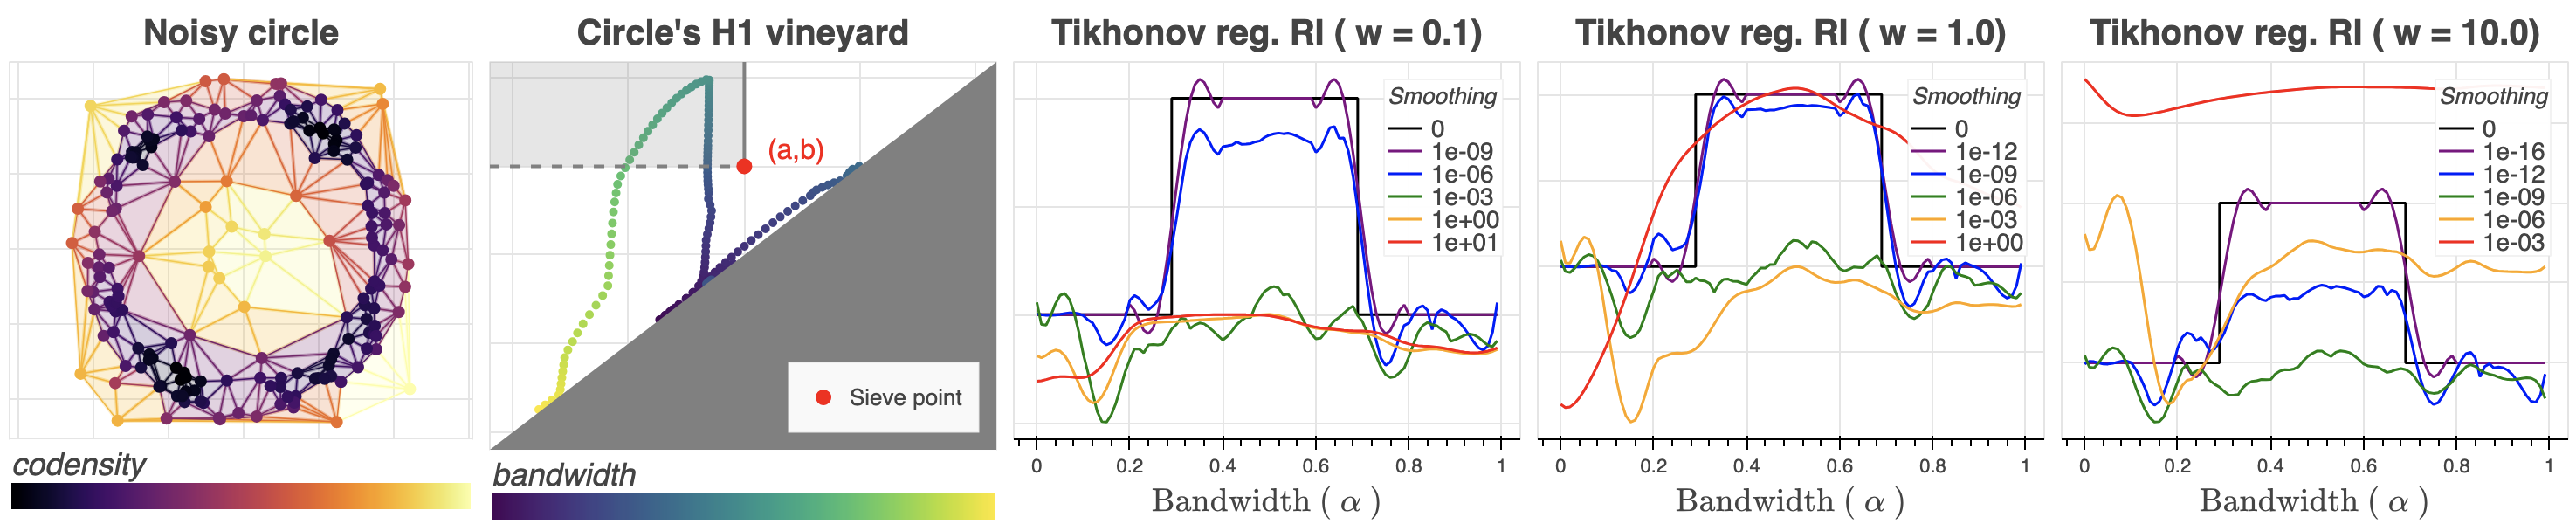
\includegraphics[width=1\linewidth,height=\textheight,keepaspectratio]{../images/codensity_ex.png}
\caption{From left to right: Delaunay complex \(K\) realized from point set \(X \subset \mathbb{R}^{2}\) sampled with multiple types of noise around \(S^{1}\) (colored by codensity at optimal \(\alpha^{\ast} \approx 1/2\)); codensity vineyard of \(\left( K,f_{\alpha} \right)\) across varying bandwidths \(\alpha\) and a fixed point \((a,b) \in \Delta_{+}\); Tikhonov relaxations \({\hat{\beta}}_{p}^{a,b}(\alpha)\) at varying regularization (\(\tau\)) and sign width (\(\omega\)) values.}
\end{figure}
Consider a Delaunay complex \(K\) realized from a point set \(X \subset \mathbb{R}^{2}\) sampled around \(S^{1}\) affected by both Hausdorff noise and strong outliers, shown in Figure~\ref{fig:codensity_opt}. One approach to detect the presence of \(S^{1}\) in the presence of such outliers is maximize \(\beta_{p}^{a,b}(\alpha)\) for some appropriately chosen \((a,b) \in \Delta_{+}\) over the pair \(\left( K,f_{\alpha} \right)\), where \(f_{\alpha}:X \rightarrow \mathbb{R}_{+}\) is a kernel (co)-density estimate:
\[\label{eq:betti_opt}
\alpha^{\ast} = \operatorname{arg\ max}\limits_{\alpha \in \mathbb{R}}\beta_{p}^{a,b}\left( K,f_{\alpha} \right),\quad\text{ where }f_{\alpha}(x) = \frac{1}{n\alpha}\sum_{i}C\left( \mathcal{K} \right)) - \mathcal{K}_{\alpha}\left. \left( x_{i} - x \right) \right.
\]
where \(C\left( \mathcal{K}_{\alpha} \right)\) is a normalizing constant that depends on the choice of kernel, \(\mathcal{K}_{\alpha}\). Intuitively, if there exists a choice of bandwidth \(\alpha^{\ast}\) which distinguishes strong outliers from Hausdorff noise clustered around \(S^{1}\), then that choice of bandwidth should exhibit a highly persistent pair \(\left. \left( a^{\ast},b^{\ast} \right) \right. \in \operatorname{dgm}_{1}\left. \left( K,f_{\alpha^{\ast}} \right) \right.\). Thus, if we place a corner point \((a,b)\) satisfying \(a^{\ast} \leq a\) and \(b < b^{\ast}\) for some \(\alpha > 0\), we expect \(\beta_{p}^{a,b}(\alpha) = 1\) to near the optimal bandwidth \(\alpha^{\ast}\)---matching the first Betti number of \(S^{1}\)---and \(0\) otherwise.

In Figure~\ref{fig:codensity_opt}, we depict the dimension-\(1\) vineyard of a simple Delaunay complex and codensity pair \(\left( K,f_{\alpha} \right)\), along with the sieve point \((a,b)\) and the region wherein \(S^{1}\) is accurately captured by persistence. As \(\beta_{p}^{a,b}\) is an integer-valued invariant, it is discontinuous and difficult to optimize; in contrast, we know from Proposition~\ref{prop:operator_props} that we can obtain a continuous and differentiable relaxation of \(\beta_{p}^{a,b}\) by replacing \(\beta_{p}^{a,b} \mapsto {\hat{\beta}}_{p}^{a,b}\) in Equation~\ref{eq:betti_opt}, enabling the use of first-order optimization techniques. By using the Tikhonov regularization from Equation~\ref{eq:tikhonov_1}, we obtain continuously varying objective curves from \({\hat{\beta}}_{p}^{a,b}(\alpha;\tau)\) which are guaranteed to have the same maxima as \(\beta_{p}^{a,b}(\alpha)\) as \(\tau \rightarrow 0\), as shown in Figure~\ref{fig:codensity_opt}. Observe lower values of \(\tau\) lead to approximations closer to the rank (black) at the cost of smoothness, while larger values can yield very smooth albeit possibly uninformative relaxations. Practical optimization of these types of objective surfaces can be handled via \emph{iterative thresholding}, a technique which alternates between gradient steps to reduce the objective and thresholding steps to enforce the rank constraints. We leave the tuning of such optimizers to future work.

\subsection{Topology-guided simplification}\label{topology-guided-simplification}

In many 3D computer graphics applications, one would like to simplify a given simplicial or polygonal mesh embedded in \(\mathbb{R}^{3}\) so as to decrease its level of detail (LOD) while retaining its principal geometric structure(s). Such simplifications are often necessary to improve the efficiency of compute-intensive tasks that depend on the size of the mesh (e.g. rendering). Though many simplification methods developed to preserve geometric criteria (e.g. curvature, co-planarity) are now well known (see \cite{heckbert1997survey} for an overview), \emph{topology-preserving} simplification techniques are relatively sparse, especially for higher embedding dimensions. Moreover, such procedures typically restrict to operations that preserve \emph{local} notions of topology, such as the genus of a feature's immediate neighborhood or the property of being a manifold. These operations are known to greatly limit the amount of detail decimation algorithms can remove.

As a prototypical application of our proposed relaxation, we re-visit the mesh simplification problem under \emph{persistence-based} constraints. In contrast to \cite{fugacci2020topology}, we forgo the use of persistence-preserving operations and instead opt for a simpler strategy: we perform an exponential search on a given sequence of simplifications, settling on the largest simplification found.

\begin{figure}
\centering
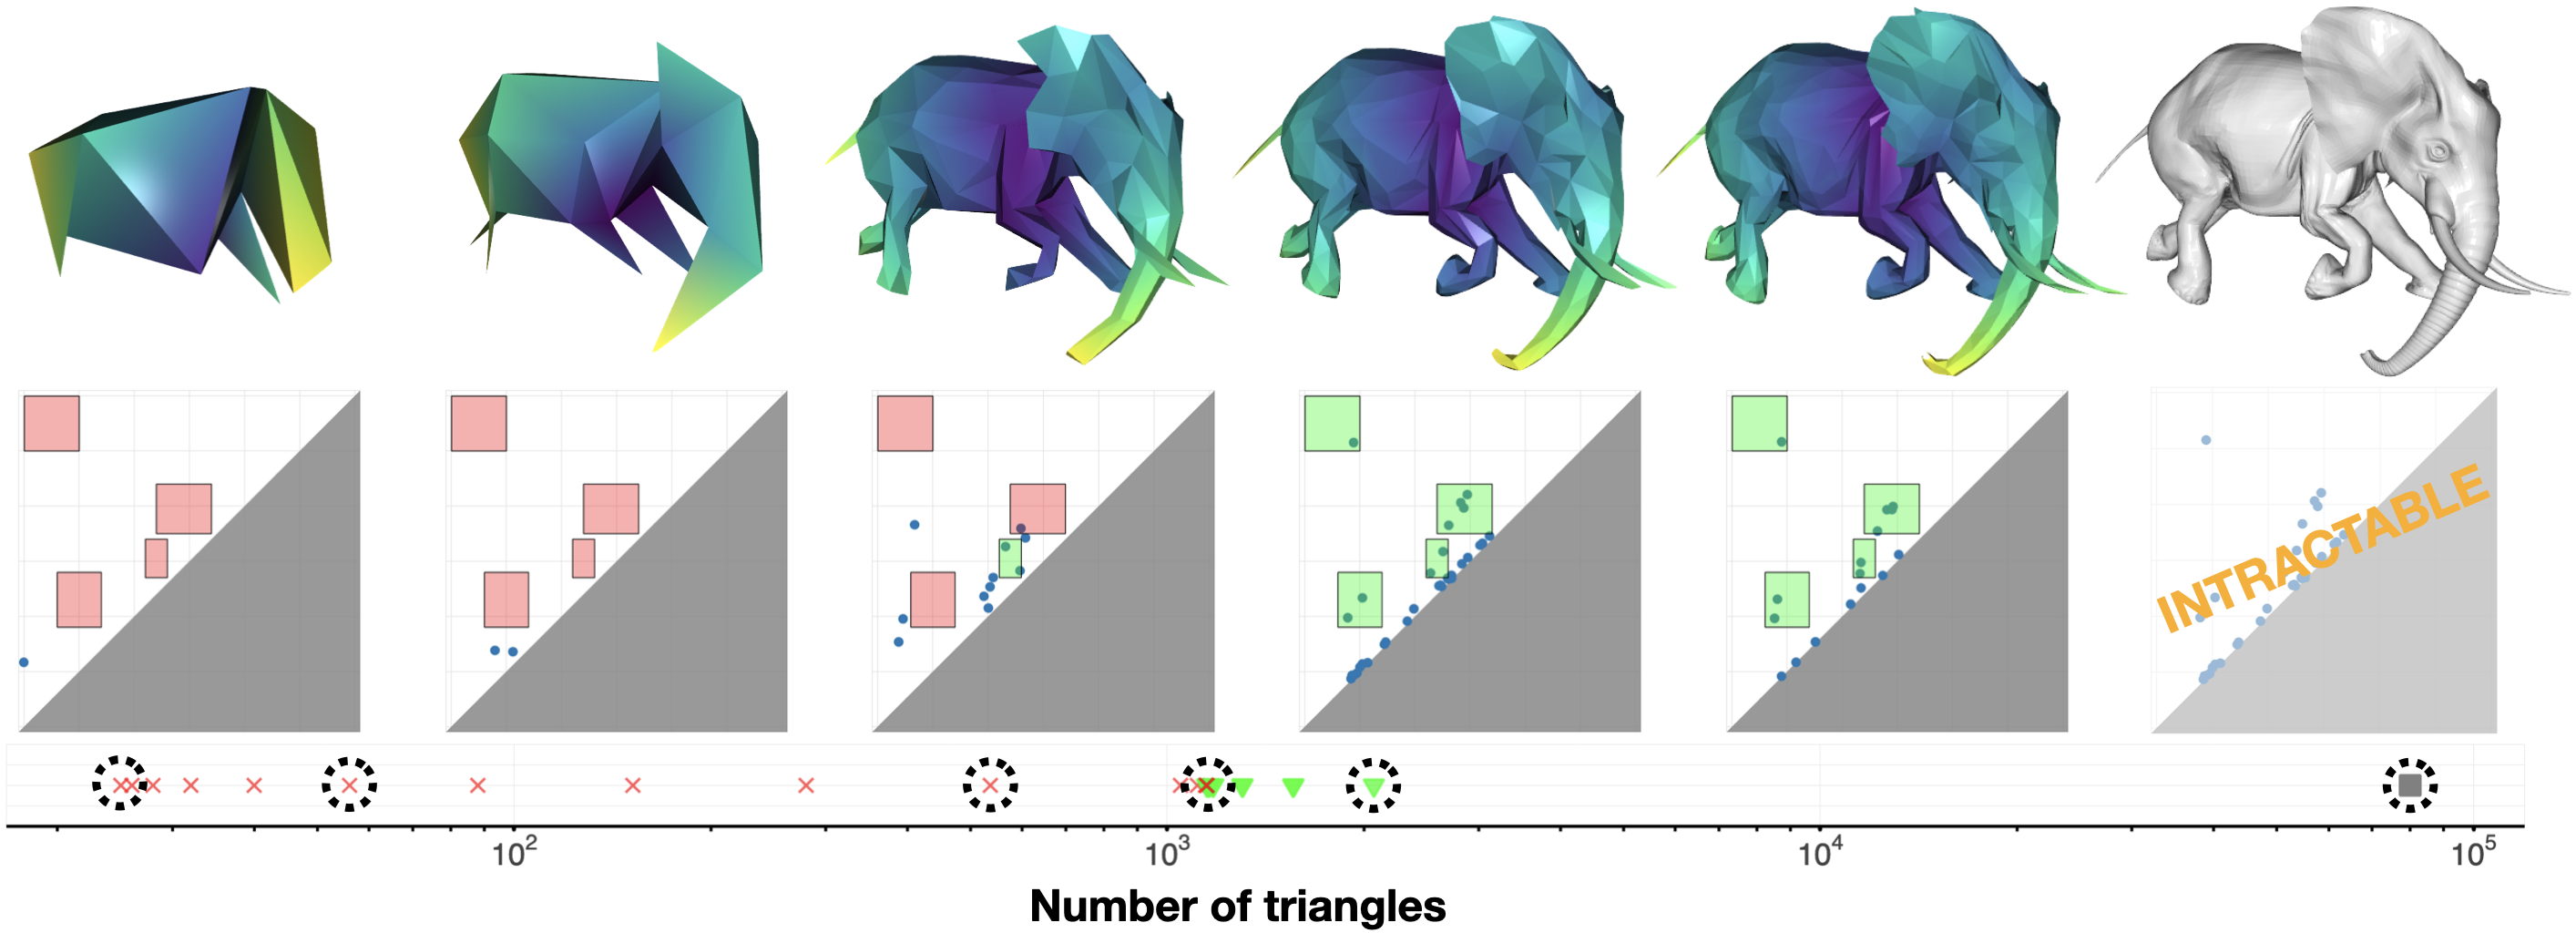
\includegraphics[width=0.95\linewidth,height=\textheight,keepaspectratio]{../images/elephant_sparsify.png}
\caption{(Top) Meshes filtered and colored by eccentricity at varying levels of simplification; (middle) their diagrams and topological constraints; (bottom) simplification thresholds tested by an exponential search, on a logarithmic scale. The color/shape of the markers indicate whether the corresponding meshes meet (green triangle) or do not meet (red x) the topological constraints of the sieve---the gray marker identifies the original mesh (not used in the search). Black dashed circles correspond with the meshes in the top row.}\label{fig:elephant_sparsify}
\end{figure}

We show an exemplary application of this idea in Figure~\ref{fig:elephant_sparsify} in sparsifying a mesh of an elephant. To filter the mesh in a geometrically meaningful way, we use the (geodesic) \emph{eccentricity} function, which assigns points \(x \in X\) in a metric space \(\left( X,d_{X} \right)\) a non-negative value representing the distance that point is from the center of the mesh:
\[\label{eq:eccentricity}
	E_{p}(x) = \left. \left( \frac{\sum_{x' \in X}d_{X}(x,x')^{p}}{N} \right) \right.^{\frac{1}{p}}
\]
\noindent To extend \(E_{p}(x)\) to simplices \(\sigma \in K\), we take the max \(f(\sigma) = \max\limits_{v \in \sigma}d_{X}(x,v)\). Note this does not require identifying a center point in the mesh. Intuitively, the highly persistent \(H_{1}\) classes in mesh carrying the most detail corresponds to ``tubular'' features that persist from the center; the four legs, the trunk, the two ears, and two tusks. In this example, four rectangular-constraints are given which ensure the simplified elephants retain these features with certain minimal persistence \(\delta > 0\).

Note that neither persistence diagrams nor deformation-compatible simplicial maps were needed to perform the sparsification, just a priori knowledge of which areas of \(\Delta_{+}\) to check for the existence of persistent topological features. We defer a full comparison of the sparsification application as future work.

\subsection{Topological time series analysis}\label{sec:topological_time_series}

The canonical lens by which time series analysis is performed is through harmonic analysis. Though mature and powerful, it can at times be more illuminating to study time series data in more geometric settings. A classical example of this is Takens delay embedding theorem, which provides sufficiency conditions under which a smooth attractor of \(d\)-dimensional manifold can be reconstructed from its dynamics \(f:M \rightarrow M\). In this context, the ``reconstruction'' is a phase space embedding of a given time series topologically equivalent to the original space, as constructed through a \emph{time-delay embedding} of \(f\):
\[
	\operatorname{SW}_{M,\tau}f(t) = ( \; f(t) \;  f(t + \tau) \; \cdots \; f(t + M\tau) \; )^{\top}
\]
\noindent where \(M + 1\) defines the \emph{embedding dimension} into \(\mathbb{R}^{M + 1}\) and \(M\tau\) is the \emph{window size} with respect to some \(\tau > 0\). Choosing different values of \(t\) yields a collection of points called the sliding window point cloud of \(f\). Under certain conditions, Takens theorem shows this reconstruction indeed has topological equivalence using the Whitney Embedding Theorem, motivating the study of the topology of \(\operatorname{SW}_{M,\tau}f\) itself. This methodology has been used to characterize non-linearity or chaotic behavior in ECG-EKG and MEG data.

The time-delay embedding requires fixing two parameters: the dimension \(M \in \mathbb{N}\) and delay \(\tau \in \mathbb{R}_{+}\). Takens theorem guarantees topological equivalence if \(M\) is more twice as large as \(d\), thus choosing dimensions larger than \(2d + 1\) poses no problems beyond sampling density and computational concerns. In contrast, once \(M\) is fixed, the embedding delay \(\tau\) strongly affects the shape of the corresponding embedding \(\operatorname{SW}_{M,\tau}\). Indeed, for general functions, the geometry of the curve \(t \mapsto \operatorname{SW}_{M,\tau}f(t)\) can be quite complicated. However, the analysis by \cite{perea2015sliding} shows that if \(f\) is periodic, the roundness\footnote{Here, \emph{roundness} is defined as the largest radius of a ball in \(\mathbb{R}^{M + 1}\) such that the curve \(\operatorname{SW}_{M,\tau}\) is tangent to at least two points from its equator.} of the sliding window point cloud is maximized as the window-size approaches the length of the period---this periodicity can be recovered by maximizing the maximum 1-dimensional persistence of the sliding window Vietoris-Rips filtration:
\[\label{eq:optimize_tau}
	\tau^{\ast} = \operatorname{arg\ max}\limits_{\tau\: \in \:\mathbb{R}_{+}}\left( \max\limits_{(a,b)\: \in \:\mathcal{D}_{\tau,f}}\left| {b - a} \right| \right),
	\quad
	\mathcal{D}_{\tau,f} = \operatorname{dgm}_{1}\left( \operatorname{Rips}(\operatorname{SW}_{M,\tau}f) \right)
\]
For more details on this connection, see Theorem 4.5 of \cite{perea2015sliding}. On the positive side, the stability of persistence alongside the Whitney embedding theorem suggests that Equation~\ref{eq:optimize_tau} is a valid proxy objective to for the purpose of detecting periodic behavior in complex or noisy signals which might otherwise be difficult to detect using e.g. autocorrelation. On the negative side, solving Equation~\ref{eq:optimize_tau} directly presents a computational complexity issue, due to the large size of \(\operatorname{Rips}\) and the high asymptotic complexity of persistence.

\begin{figure}
\centering
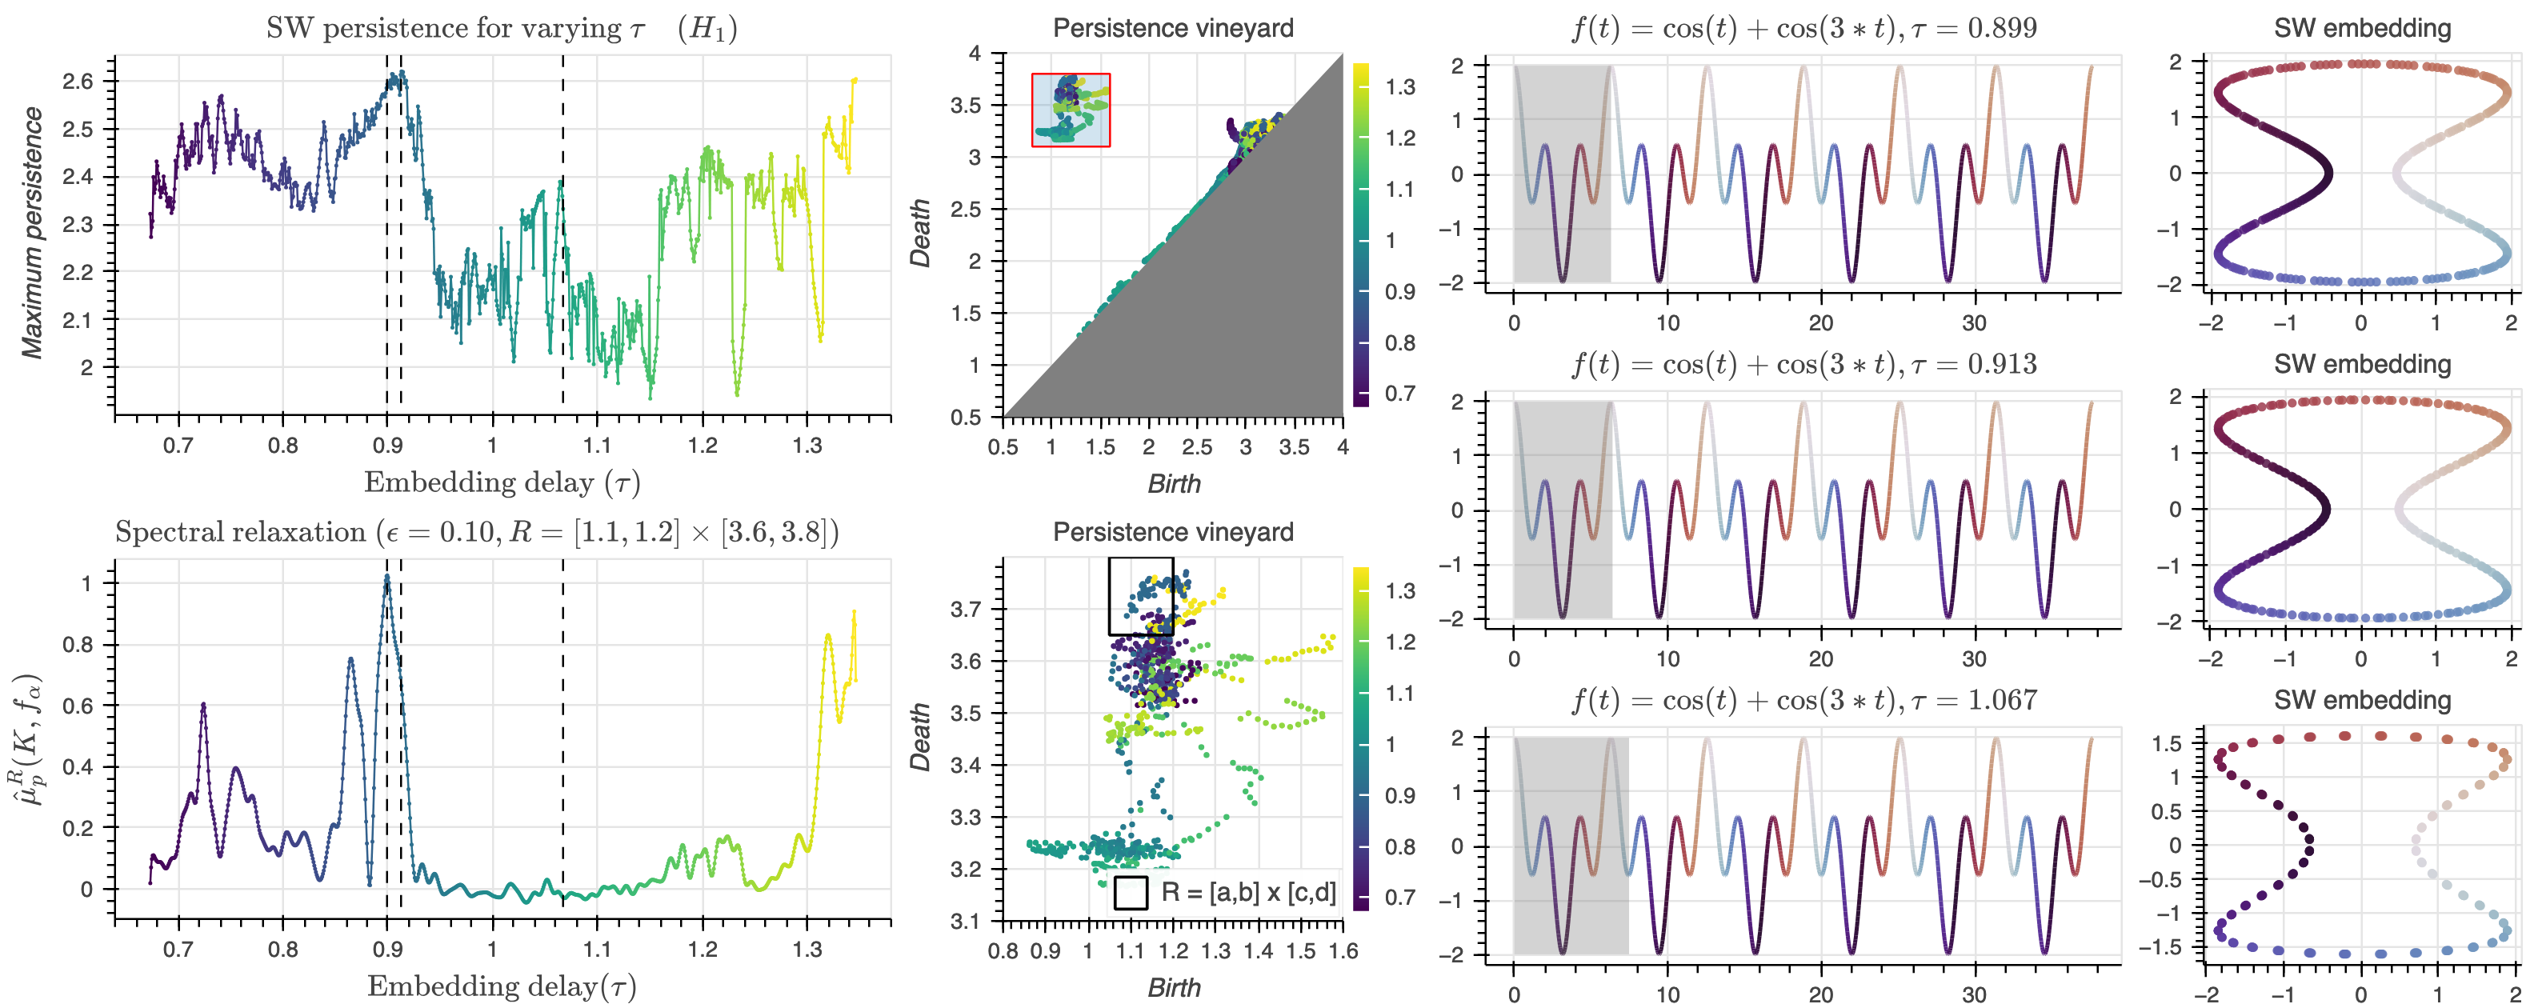
\includegraphics[width=1\linewidth,height=\textheight,keepaspectratio]{../images/sw1pers_mu.png}
\caption{Maximum SW 1-persistence for \(\mathcal{D}_{\tau,f}\) at varying \(\tau \in \lbrack 2\pi c/8,2\pi c/4\rbrack\) with \(c = 7/8\) alongside the spectral multiplicity \({\hat{\mu}}_{p}^{R}\left( K,f_{\alpha} \right)\) for regularization \(\varepsilon = 0.10\) and box \(R = \lbrack 1.1,1.2\rbrack \times \lbrack 3.6,3.8\rbrack\) (left); two vineyard plots, one showing the region that determines maximum persistence (middle-top), the bottom showing the chosen box \(R\) (middle-bottom); time series \(f(t)\) with window-lengths \(M\tau\) highlighted for three values of \(\tau\) and their embedding plotted with PCA (right).}\label{fig:sw1pers_spirit}
\end{figure}

To illustrate another application of our spectral relaxation, we consider an proxy optimization problem that is both easier and more efficient to optimize than Equation~\ref{eq:optimize_tau}. We begin with a simple periodic function \(f\) given by:
\[
f(t) = \cos(t) + \cos(3t),\quad t \in \lbrack 0,12\pi\rbrack
\]
Regarding the parameterization, we consider optimizing \(\tau\) over the interval \(\lbrack 2\pi c/8,2\pi c/4\rbrack\) using the Tikhonov regularized spectral multiplicity \({\hat{\mu}}_{p}^{R}\) with a (large) regularization from Equation~\ref{eq:tikhonov_1} with \(\varepsilon = 0.10\). To determine the proxy objective function \({\hat{\mu}}_{1}^{R}\), we fix a rectangle \(R = \lbrack 1.1,1.2\rbrack \times \lbrack 3.6,3.8\rbrack \in \Delta_{+}\), which we determined contains the correct maximizer by inspection of the persistence vineyard\footnote{In practice, the full vineyard wouldn't be available, and the box \(R\) would need to be determined using apriori knowledge or by probing random subsets of \(R \subset \Delta_{+}\) for non-trivial persistence.}. All other parameters determined, we plot both the (true) maximum persistence and the optimization surface of \({\hat{\mu}}_{1}^{R}\) on the top and bottom left subplot of Figure~\ref{fig:sw1pers_spirit}, respectively.

Analogous to the Takens and Nyquist-Shannon theorems, \cite{perea2015sliding} show that for trigonometric polynomials, one loses no information if the embedding dimension is greater than twice the maximum frequency, thus we set \(M = 7\) and sample \(n = 300 \gg 2(3 \cdot 6)\) points to ensure no issues related dimension or sampling density occur. Then, we measure the maximum dimension-1 persistence of \(\mathcal{D}_{\tau,f}\) across 900 equispaced delay values \(\tau \in \lbrack 0,12\pi\rbrack\), which we plot on the top left of Figure~\ref{fig:sw1pers_spirit}. We observed the maximum persistence was attained at around \(\tau \approx 0.913\); the theory from \cite{perea2015sliding} suggests that if \(f\) is \(L\)-periodic, the delay value \(\tau\) which achieves the maximum persistence should be around \(\tau = 2\pi c/L \approx 0.916\) where \(c = M/(M + 1)\) is the proportionality constant.

\subsection{Low memory persistence computations}\label{sec:low_memory}

One particular limitation of the persistence computation is its space usage. Though the initial boundary matrices (when explicitly constructed) are known to be sparse, both the constitutive matrices storing the reduced boundary chains (\(R\)) and the cycle representatives (\(V\)) are known to lose their sparsity throughout the duration of the reduction. As the number of non-zeros in \(R\) affects the performance of reduction, analyzing the worst and average-case amount of ``fill-in'' is a subject of recent research \cite{bauer2022keeping}. Though the average case complexity is far better than the worst case, space usage is a well known to be one of the barriers antagonizing the scalability of the persistence computation. As the persistence diagram may be entirely determined by rank computations, the time and space complexity results from Proposition~\ref{prop:spectral_rank_complexity} extend directly to the computation of persistence diagrams via Chen and Kerbers divide-and-conquer approach \cite{chen2013output}.

\begin{figure}
\centering
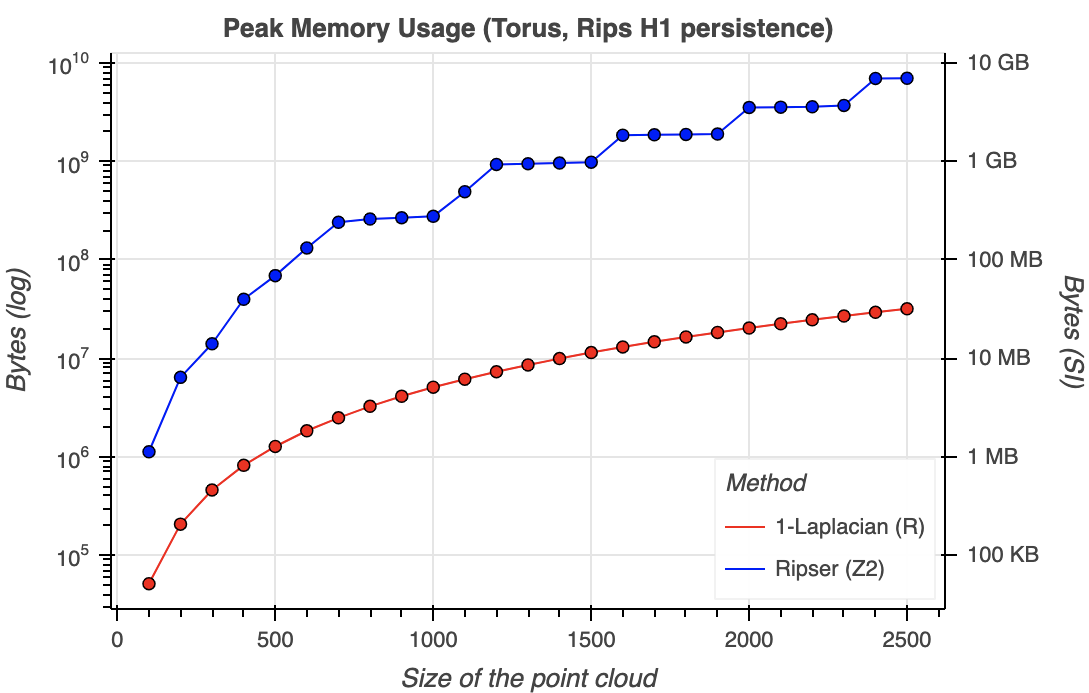
\includegraphics[width=0.65\linewidth,height=\textheight,keepaspectratio]{../images/ripser_vs_laplacian.png}
\caption{(Blue) The ``high watermark'' maximum (heap) memory allocated by Ripser in computing persistence of a Rips filtration \(K\) up to the enclosing radius. (Red) the maximum memory allocated by the Jacobi matrix constructed from a degree-\(|K|\) Lanczos expansion of \(\mathcal{L}_{p}(K)\). Note that the Jacobi matrix of \(\mathcal{L}_{p}(K)\) (or of some subset thereof) contains all the information needed to reconstruct the persistence invariants.}
\end{figure}

\phantomsection\label{fig:ripser_vs_laplacian}{}

To demonstrate the space efficiency of the matrix-free approach, we revisit the persistence computation in the context of the homology inference problem, one of the original use-cases of persistence \cite{perea2018brief}. To measure the scalability of the Lanczos method, we measure its space usage via the persistence computation on an increasingly dense point cloud sampled from the uniform measure on the 2-torus \(\mathbb{T}\) (via \cite{diaconis2013sampling}): 
\[
f(\theta,\varphi) = \left( \left( R + r\cos(\theta) \right)\cos(\varphi),\left( R + r\cos(\theta) \right)\sin(\varphi),r\sin(\theta) \right)
\]
\noindent
To ensure uniform coverage of \(\mathbb{T}\), we build the point clouds using \(k\)-prefixes of the \emph{greedy permutation} of a dense point sample, for \(k\) varying along evenly spaced points from \(50\) to \(2500\) (yielding complexes with sizes ranging from \(2.0 \cdot 10^{4}\) to \(2.6 \cdot 10^{9}\) simplices, respectively). For each \(k\), we compute both the persistence of the Rips filtration \(K\) up to the enclosing radius using the popular software \emph{Ripser} \cite{bauer2021ripser} and the Jacobi matrix of the \(K\)`s corresponding combinatorial Laplacian using the Lanczos method, up to degree \(|K|\). To maximize space efficiency, like \emph{Ripser}, we use the \emph{apparent pairs} optimization to discard zero-persistence pairs (see Section~\ref{sec:apparent-pairs-optimization}). For a fair comparison in terms of space usage, we record the maximum (heap) memory allocated by tracing all system allocations using the software \emph{Memray}\footnote{See \url{https://bloomberg.github.io/memray/memory.html} for an overview of how memory is measured.}.

It's worth noting the results in Figure~\ref{fig:ripser_vs_laplacian} carry certain limitations. In particular, we only report the memory usage of both methods, rather than the time usage, as the method by Chen and Kerber has simply too large of an compute overhead to be practical. Additionally, \emph{Ripser} is computing persistence here with respect to \(\mathbb{Z}/2\) coefficients, whereas we rely on IEEE 64-bit floating precision arithmetic as a proxy for \(\mathbb{R}\) (thus the persistence diagrams are not identical). For more limitations, see Section~\ref{sec:concluding-remarks}.

\subsection{Shape comparison via featurization}\label{sec:shape_comparison}

Analogous to its historical use in comparing shapes (i.e. manifolds, curves, etc.) through size functions, persistence has increasingly found use in machine learning pipelines through the use of mappings from diagrams to function spaces (e.g. Hilbert spaces). One notable such featurization is the persistent homology transform (PHT) \cite{turner2014persistent}, an injective transform which filters a triangulated space \(\mathcal{X}\) embedded in \(\mathbb{R}^{d}\) via the sublevel set parameterization \({\mathcal{X}(v)}_{r} = \left\{ x \in \mathcal{X}:x \cdot v \leq r \right\}\), where \(v \in S^{d - 1}\). The intuition here is that by ``looking'' at the sublevel-set persistence of the shape \(\mathcal{X}\) from all possible directions \(v \in S^{1}\), one can recover enough information to fully reconstruct \(\mathcal{X}\) from the collection of diagrams alone.

\begin{figure}
\centering
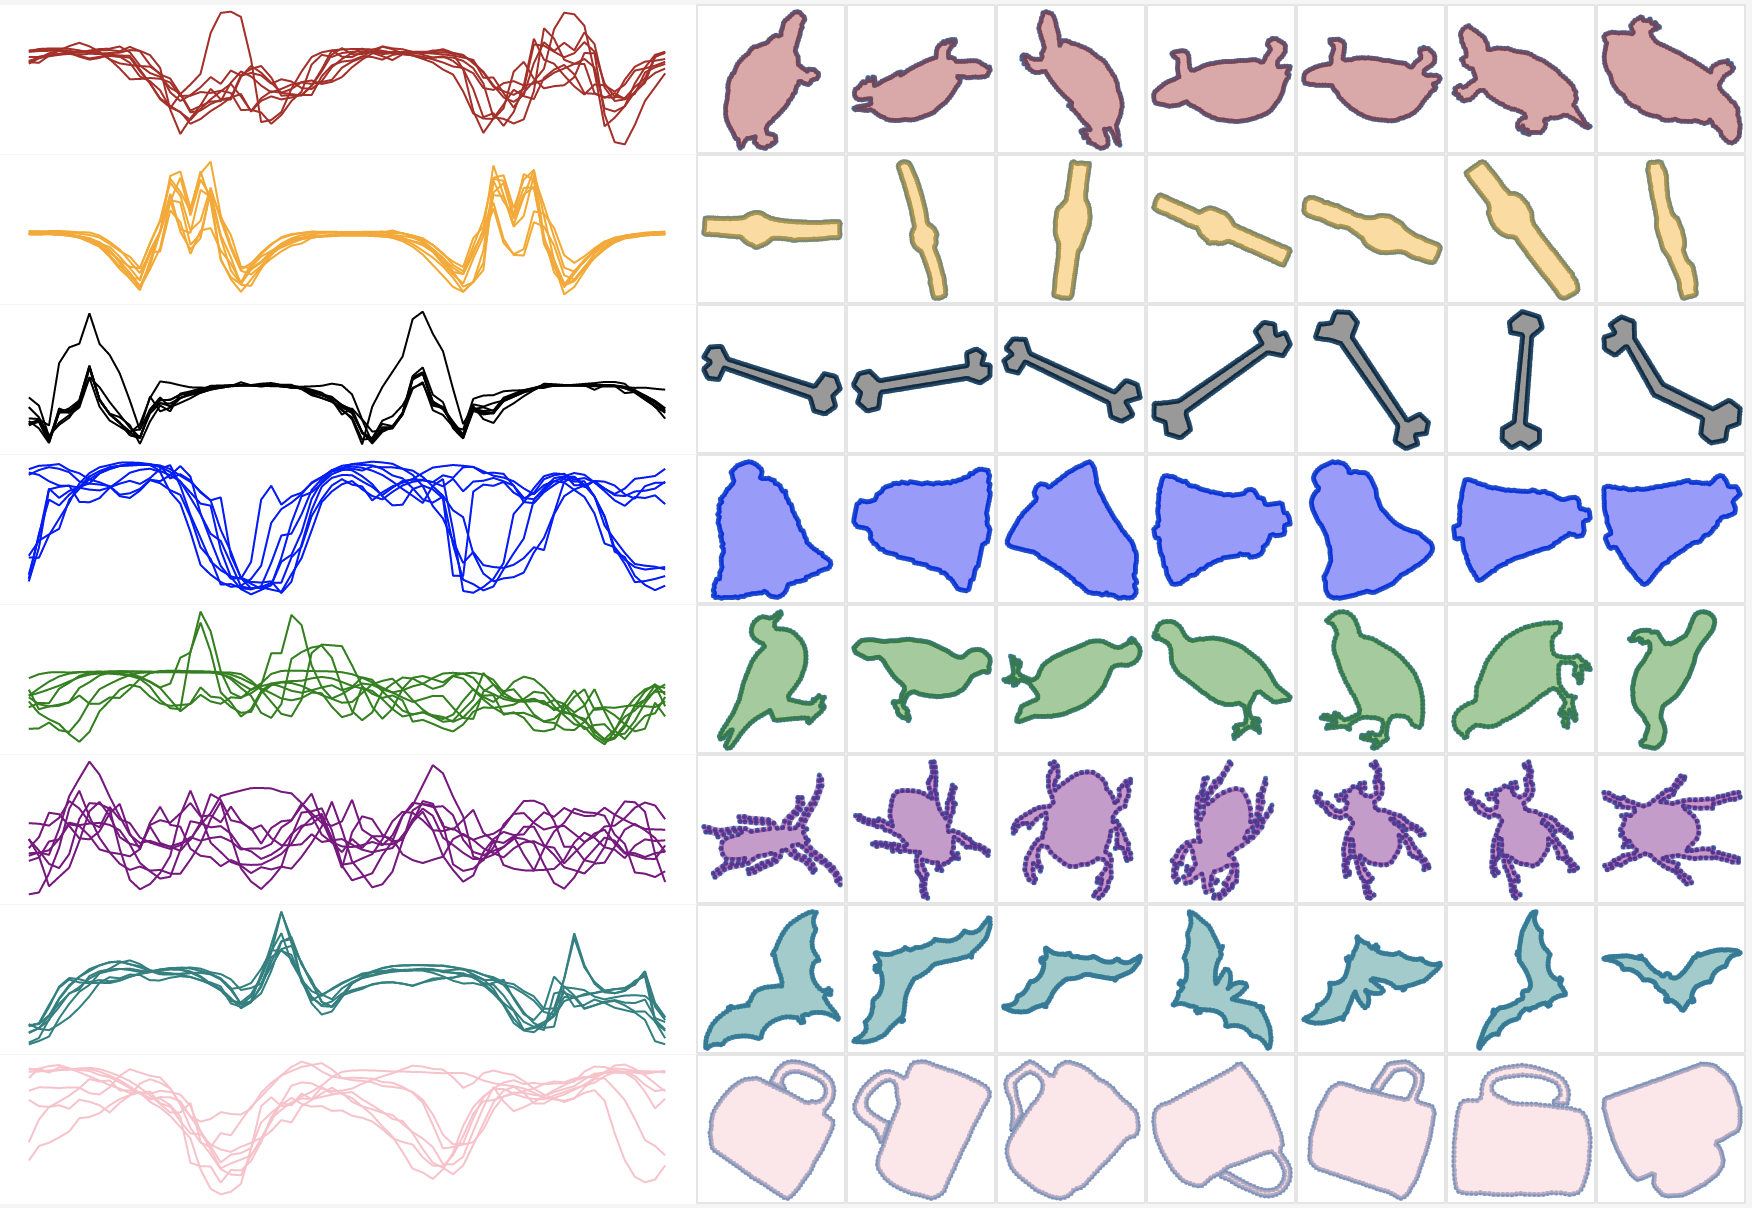
\includegraphics[width=0.65\linewidth,height=\textheight,keepaspectratio]{../images/mpeg7_heattrace.png}
\caption{Spectral signatures generated from filtering combinatorial Laplacians of MPEG7 2D shape datasets using the directional transform. By using the relaxation from Equation~\ref{eq:heat_sf}, these signatures can be interpreted as combinations of heat traces over the interval \(\lbrack 0,2\pi)\). Observe that highly similar shapes generate curves that maintain a large degree of intra-class similarity under the \(\ell_{2}\) norm whereas outliers are detected and retain dissimilarity between classes (e.g. the bent bone in the black class exhibits higher peaks in it signature compared to its class, but is highly class-similar.)}\label{fig:mpeg7_curves}
\end{figure}

Aside from sparking an inverse theory for persistence, the injectivity of the PHT also provides the foundation necessary for equipping shape spaces with bona fide distance metrics. For example, one such metric is given by the integrated Wasserstein distance \(\operatorname{dist}_{\mathcal{X}}\) between the sublevel-set persistence diagrams \(\operatorname{dgm}_{p}(X,v)\):
\[
\operatorname{dist}_{\mathcal{X}}(X,X') = \sum_{p = 0}^{d}\int_{S^{d - 1}}d_{W}\left( \operatorname{dgm}_{p}(X,v),\operatorname{dgm}_{p}(X',v) \right)dv
\]
\noindent where \(X,X' \in \mathcal{X}\). In most machine learning applications, distance metrics are often difficult---if not intractable--to analytically determine; instead, most practitioners either craft or learn task-specific pseudometrics that are easy to compute and discriminative enough for the given application.

We seek to learn shape-sensitive, discriminative pseudometrics from weaker persistence invariants. Towards this end, consider the following parameterization, for some fixed simplicial complex \(K\) and pair \((a,b) \in \Delta_{+}\):
\[
\begin{aligned}
\mathcal{B}_{a,b}: & \; S^{d - 1} & \rightarrow & \; \mathbb{R} \\
 & \; v & \mapsto & \; \beta_{p}^{a,b}(X,v)
\end{aligned}
\] 
\noindent where \(\beta_{p}^{a,b}(X,v) = \left| \left\{ (a',b') \in \operatorname{dgm}_{p}(K,v):a' \leq a,b < b' \right\} \right|\). When \(d = 2\), this is a piecewise-constant function periodic over the interval \(\lbrack 0,2\pi)\). The collection of all such curves over \(\Delta_{+}\) characterizes all the information in PHT, thus it is a natural candidate hypothesis space for learning algorithms. However, some choices of pairs \((a,b) \in \Delta_{+}\) may yield functions which have little-or-no information (e.g. identically zero or constant functions), suggesting that some choices of \((a,b) \in \Delta_{+}\) may be more useful than others for the purpose of classification.

To demonstrate another application of our methodology for shape classification, we apply our spectral relaxation to the MPEG-7 shape matching data set from \cite{bai2009learning}. To build a classifier, we generate curves \(\mathcal{B}_{a,b} = \{ {\hat{\beta}}_{p}^{a,b}(K,v) : v \in S^{1} \}\) for random  \((a,b) \in \Delta_{+}\), which act as hypotheses functions \(h_{\ast}(x)\) in an ensemble model \(H\):
\[
	H(x) = \mathrm{sign}\left( \alpha_{1}h_{1}(x) + \alpha_{2}h_{2}(x) + \cdots + \alpha_{t}h_{t}(x) \right)
\]
\noindent
To determine the coefficients \(\alpha_{\ast}\), we use the classical AdaBoost method~\cite{mukherjee2013rate}, sampling new hypothesis functions \(h_{\ast}\) uniformly at random from a bounded subset of \(\Delta_{+}\). We choose the spectral relaxation \(\phi(\lambda,\tau) = 1 - \exp( - \lambda/\tau)\) with a smoothing parameter \(\tau = 1 \cdot 10^{- 1}\). Following Equation~\ref{eq:heat_sf}, the corresponding curves \(\mathcal{B}_{a,b}\) may be interpreted as combinations of \emph{heat kernel traces}, which are known to be useful for characterizing graphs \cite{xiao2009graph}.

In Figure~\ref{fig:mpeg7_curves}, we plot the curves associated to one such hypothesis function generated for the ensemble. Observe that highly similar shapes generate curves that maintain a large degree of intra-class similarity under the \(\ell_{2}\) norm whereas outliers are detected and retain dissimilarity between classes (e.g. the bent bone in the black class exhibits higher peaks in it signature compared to its class, but is highly class-similar). This suggests that, for some choice \((a,b) \in \Delta_{+}\) and certain choices of \(\phi\), composing the spectrally-relaxed persistent rank function with the direction transform is viable strategy for generating \emph{weak learners} for machine learning purposes.

\section{Concluding Remarks and Limitations}\label{sec:concluding-remarks}

In summary, we have introduced various spectral relaxations of the persistent rank function, which has a wealth of useful properties, including differentiability on the positive semi-definite cone, a matrix-free representation, and natural connections to variational constructions common in machine learning applications, such as the Tikhonov regularization and the Heat kernel. By focusing on coefficients in \(\mathbb{R}\), we were able to exploit the connection between the inner product spaces on cochain spaces and the theory of persistence measures, providing an avenue to introduce diffentiability to an otherwise discontinuous function. Moreover, by focusing on the spectral characterization of the rank function, we were able to study persistence in the setting of \emph{iterative methods}, a pursuit which lead us to the Lanczos method of Krylov expansion. Surprisingly, these computational techniques turned out to pair well with the output-sensitive algorithm from \cite{chen2011output}, which we demonstrated may be used to compute \(\Gamma\)-persistence pairs in an output sensitive fashion. As cycle representatives can be obtained once a pairing has been constructed, the iterative approach may be used to compute essentially any persistence invariant.

\subsection{Limitations}\label{sec:limitations}

There are few limitations to the proposed work that may prevent its practical use, depending on the problem and invariant of interest. We mention the limitations to the approaches proposed that we are aware of below.
\\
\\
\noindent \textbf{Function parameterization}: Choosing the matrix function \(\Phi\) from Equation~\ref{eq:lowner} and tuning any of its associated hyper-parameters (i.e. \(\tau\) and \(\omega\) ) can be very application-dependent. We demonstrate this in Figure~\ref{fig:codensity_opt} ---for some values of \(\tau > 0\), the relaxation can be either have high variance due to instability or high bias due over smoothing. In the optimization setting, we addressed these issues via an iterative shrinkage approach; in the more general setting, these choices depend on a multitude of factors, such as the relative precision the target invariant needs to achieve, the amount of compute resources available, etc. 
\\
\\
\noindent \textbf{Rank instability}: Though the persistence rank invariant is considered a ``stable function'' in the multi-parameter setting \cite{cerri2013betti}, this stability is generally proven by reduction to a matching-type distance between the pairings themselves. In particular, the Betti number function \(\beta_{p}^{\ast}\) and its various related invariants---such as the sequence containing the Betti numbers of the homology groups at all scales (the ``\emph{Betti sequence}'')---is in fact \emph{unstable} with respect to the \(1\)-Wasserstein distance (see Theorem 2.5 in \cite{johnson2021instability}). We sought to address this instability by a spectral approach, but other approaches that could be used; for example, both~\cite{johnson2021instability} and~\cite{adams2017persistence} provide a Gaussian-smoothing type stabilization procedure, though they also both require access to the pairings. Another approach---which depends only on the rank---is the \emph{hierarchical stabilization} method from \cite{gafvert2017stable}, though this remains unexplored.
\\
\\
\noindent \textbf{Randomized estimation:} Computing some of the persistence invariants exactly---such as the pairing itself---poses some difficult in practice, especially when the exact rank is required. For example, in the divide-and-conquer algorithm from \cite{chen2011output}, a single wrong rank value can lead to unpredictable output. If a randomized estimator with fixed success probability \(p > 0\) is used, then one may need to be re-run \(k\) times to achieve a higher success probability \(\left( 1 - (1 - p)^{k} \right)\). Fortunately, for any constant \(\delta \in (0,1)\), Lemma 10 of \cite{chen2011output} shows the number of such rank computations needed to compute \(\Gamma\)-persistent pairs is not larger than:

\[\rho = \rho(n,\left\lceil \frac{1}{\delta} \right\rceil) = 4n\left. \left( 2\left\lceil \frac{1}{\delta} \right\rceil + \log n + 1 \right) \right.\]

\noindent Indeed, the analysis from section 6 of \cite{chen2011output} shows that if the rank estimator has success probability \(p\) and \(\hat{p} = 1 - p\), then for the entire algorithm to achieve an arbitrary success probability \(q > 0\), every rank computation needs to be repeated at most \(k\) times, where:
\[
{\log(1/\hat{p})}^{- 1} \cdot \log(\omega) \leq k,\quad\omega = \left( 1 - q^{\frac{1}{\rho}} \right)^{- 1}
\]
\noindent Since \(\log(\omega) = \Theta(\rho)\), every rank computation requires \(O\left( \log\rho \right) = O\left( \log n + \log\frac{1}{\delta} \right)\) repeated trials. In other words, the randomized aspect of the algorithm does not significantly affect its computational complexity, though it does increase the complexity of a practical implementation.
\\
\\
\textbf{Estimator efficiency:} In theory, perhaps the largest limitation of approximating the rank function via the GH Monte-carlo estimator via Equation~\ref{eq:gh_trace_estimator} is its convergence rate, which is dominated by \(O\left( \epsilon^{- 2} \right)\). If \(\epsilon\) is small, the number of iterations the estimator needs to \emph{provably} obtain a \((1 \pm \epsilon)\)-approximation can be astronomical. To make matters worse, estimating the numerical rank may requires shrinking \(\epsilon\) to the order of \(O(1/n)\). Thus its practical utility lies in applications where \(\epsilon\) need not be too small, i.e. only a relatively coarse approximation of \(\operatorname{tr}\left( f(A) \right)\) is needed. From our view, this slow convergence and high precision combination of the GH estimator Equation~\ref{eq:gh_trace_estimator} is the only major barrier preventing the use of matrix-free techniques in more practical application settings.

In practice, the efficiency of the iterative implicit trace estimator from Section~\ref{sec:iterative_approx} depends on a variety of nuanced factors, such as the condition number of the operator, the spectral gap, etc. Fortunately, implicit trace estimation is active area of research; recent results by Meyers et al. \cite{meyer2021hutchpp}, for example, show how the estimator Equation~\ref{eq:gh_trace_estimator} can be modified to obtain a \(\left. (1 \pm \epsilon) \right.\) approximation using only \(O\left( \varepsilon^{- 1} \cdot \sqrt{\log\left( \eta^{- 1} \right)} + \log\left( \eta^{- 1} \right) \right)\) samples using deflation techniques, though this does require additional re-orthogonalization and storage costs. Even more recently, optimal trace estimators based on the \emph{exchangeability principle} and the \emph{Nyström approximation} have been shown to not only match the \(O\left( 1/n^{2} \right)\) variance reduction rate of Hutch++, but to also empirically achieve much faster convergence \cite{epperly2024xtrace}.

Interestingly, using a reduction to the Gap-Hamming problem, it was shown that achieving a \((1 \pm \epsilon)\) trace approximation with probability greater than \(3/4\) requires at least \(\Omega(\epsilon^{- 1})\) matrix-vector queries \(v \mapsto Av\) if the input vectors \(v \in \mathbb{R}^{n}\) are chosen \emph{non-adaptively} \cite{meyer2021hutchpp} (i.e. independent of the structure of \(A\)). This lower bound suggests it may be possible to achieve a \(O(1 \pm \epsilon)\) approximation of the rank-based invariants from Proposition~\ref{prop:spectral_rank_complexity} with the same space complexity and without exact arithmetic, but no algorithm is known to the author that achieves this non-adaptive bound.

\backmatter
\bmhead{Supplementary information}
\bmhead{Acknowledgements}
\section*{Declarations}

%Some journals require declarations to be submitted in a standardised format. Please check the Instructions for Authors of the journal to which you are submitting to see if you need to complete this section. If yes, your manuscript must contain the following sections under the heading `Declarations':
%
%\begin{itemize}
%\item Funding
%\item Conflict of interest/Competing interests (check journal-specific guidelines for which heading to use)
%\item Ethics approval and consent to participate
%\item Consent for publication
%\item Data availability 
%\item Materials availability
%\item Code availability 
%\item Author contribution
%\end{itemize}

\begin{appendices}

\section{}\label{sec:appendix}

\subsection{Proofs}\label{sec:proofs}

\begin{proof}[Proof of Lemma Lemma~\ref{lemma:rank}]
	\setlength{\abovedisplayskip}{1em}
	\setlength{\belowdisplayskip}{1em}
	The Pairing Uniqueness Lemma\cite{edelsbrunner2000topological} asserts that if $R = \partial V$ is a decomposition of the total $m \times m$ boundary matrix $\partial$, then for any $1 \leq i < j \leq m$ we have $\mathrm{low}_R [j] = i$ if and only if $r_\partial (i , j) = 1$. As a result, for $1 \leq i < j \leq m$, we have: 
\[
	\mathrm{low}_R [j] = i \Leftrightarrow r_R (i , j) \neq 0 \Leftrightarrow r_\partial (i , j) \neq 0
\]
Extending this result to Equation~\ref{eq:lower_left_rank} can be seen by observing that in the decomposition, $R = \partial V$, the matrix $V$ is full-rank and obtained from the identity matrix $I$ via a sequence of rank-preserving (elementary) left-to-right column additions.
\end{proof}

\begin{proof}[Proof of Proposition~\ref{prop:mu_betti_1}]\label{proof:mu_betti_1}
	\setlength{\abovedisplayskip}{1em}
	\setlength{\belowdisplayskip}{1em}
	We first need to show that $\beta_p^{i, j}$ can be expressed as a sum of rank functions. Note that by the rank-nullity theorem, so we may rewrite Equation~\ref{eq:pbn} as: 
	\[
	\beta_p^{i, j} = \mathrm{dim}(C_p (K_i)) - \mathrm{dim}(B_{p - 1} (K_i)) - \mathrm{dim}(Z_p (K_i) \cap B_p (K_j))
	\] 
	The dimensions of groups $C_p (K_i)$ and $B_p (K_i)$ are given directly by the ranks of diagonal and boundary matrices, yielding: 
	\begin{displaymath}
		\beta_p^{i, j} = \mathrm{rank}(I_p^{1, i}) - \mathrm{rank}(\partial_p^{1, i}) - \mathrm{dim}(Z_p (K_i) \cap  B_p (K_j)) 
	\end{displaymath}
	To express the intersection term, note that we need to find a way to express the number of $p$-cycles born at or before index $i$ that became boundaries before index $j$. 
	Observe that the non-zero columns of $R_{p+1}$ with index at most $j$ span $B_p (K_j)$, i.e. $\{\; \mathrm{col}_{R_{p+1}}[k] \neq 0 \mid k \in [j] \;\} \in \mathrm{Im}(\partial_{p+1}^{,j})$. 
	Now, since the low entries of the non-zero columns of $R_{p+1}$ are unique, we have: 
	\[\label{eq:s1}
	\mathrm{dim}(Z_p (K_i) \cap B_p (K_i)) = \lvert \Gamma_p^{i,j} \rvert 
	\]
	where $\Gamma_p^{i,j} = \{\; \mathrm{col}_{R_{p+1}}[k] \neq 0 \mid 1 \leq \mathrm{low}_{R_{p+1}} [k] \leq i \}$. Consider the complementary matrix $\bar{\Gamma}_p^{i,j}$ given by the non-zero columns of $R_{p+1}$ with index at most $j$ that are not in $\Gamma_p^{i,j}$, i.e. the columns satisfying $\mathrm{low}_{R_{p+1}}[k] > i$. Combining rank-nullity with the observation above, we have: 
	\[\label{eq:s2}
	\bar{\Gamma}_p^{i,j} = \mathrm{dim}(B_p (K_j)) - \lvert \Gamma_p^{i,j} \rvert = \mathrm{rank}(R_{p+1}^{i+1,j}) 
	\]
	Combining equations Equation~\ref{eq:s1} with Equation~\ref{eq:s2} yields:
	\[\label{eq:s3}
	\mathrm{dim}(Z_p(K_i) \cap B_p(K_j)) = \lvert( \Gamma_p(i,j)) = \mathrm{dim}(B_p (K_j)) - \lvert \bar{\Gamma}_p^{i,j} \rvert  = \mathrm{rank}(R_{p+1}^{1,j}) - \mathrm{rank}(R_{p+1}^{i+1,j}) 
	\]
	\noindent Observing the final matrices in Equation~\ref{eq:s3} are \emph{lower-left} submatrices of $R_{p+1}$, the final expression Equation~\ref{eq:betti_four} follows by applying Lemma~\ref{lemma:rank} repeatedly. 
\end{proof}


\subsection{Combinatorial Laplacians}\label{sec:laplacian_theory}

The natural extension of the graph Laplacian \(L\) to simplicial complexes is the \emph{\(p\)-th combinatorial Laplacian} \(\Delta_{p}\), whose explicit matrix representation is given by Equation~\ref{eq:comb_lap}. Indeed, when \(p = 0\), \(\Delta_{0}(K) = \partial_{1}\partial_{1}^{T} = L\) recovers the graph Laplacian. As with boundary operators, \(\Delta_{p}(K)\) encodes simplicial homology groups in its nullspace, a result known as the discrete Hodge Theorem~\cite{lim2020hodge}:
\[
{\widetilde{H}}_{p}\left( K;\mathbb{R} \right) \simeq \ker\left( \Delta_{p}(K) \right),\quad\beta_{p} = \operatorname{nullity}\left( \Delta_{p}(K) \right)
\]
\noindent The fact that the Betti numbers of \(K\) may be recovered via the nullity of \(\Delta_{p}(K)\) has been well studied (see e.g. Proposition 2.2 of \cite{horak2013spectra}). In fact, one need not only consider \(\Delta_{p}\) as the spectra of \(\Delta_{p}\), \(L_{p}^{\operatorname{up}}\), and \(L_{p}^{\operatorname{dn}}\) are intrinsically related by the identities:
\[
\Lambda\left( \Delta_{p}(K) \right) \doteq \Lambda\left. \left( L_{p}^{\operatorname{up}} \right) \right. 
\cupdot
\Lambda\left. \left( L_{p}^{\operatorname{dn}} \right) \right.,\quad\quad\Lambda\left. \left( L_{p}^{\operatorname{up}} \right) \right. \doteq \Lambda\left. \left( L_{p + 1}^{\operatorname{dn}} \right) \right.\]
\noindent where \(A \doteq B\) and \(A \cupdot B\) denotes equivalence and union between the \emph{non-zero} elements of the multisets \(A\) and \(B\), respectively, counted with multiplicity. Moreover, all three operators \(\Delta_{p}\), \(L_{p}^{\operatorname{up}}\), and \(L_{p}^{\operatorname{dn}}\) are symmetric, positive semidefinite, and compact---thus, for the purpose of estimating \(\beta_{p}\), it suffices to consider only one family of operators.

\subsection{Laplacian matvec}\label{app:lap_matvec}

Given a simple undirected graph \(G = (V,E)\), let \(A \in \{ 0,1\}^{n \times n}\) denote its binary adjacency matrix satisfying \(A\left. \lbrack i,j\rbrack \right. = 1 \Leftrightarrow i \sim j\) if the vertices \(v_{i},v_{j} \in V\) are adjacent in \(G\), and let \(D = \operatorname{diag}\left. \left( \{\,\deg\left( v_{i} \right)\,\} \right) \right.\) denote the diagonal \emph{degree} matrix, where \(\deg\left( v_{i} \right) = \sum_{j \neq i}A\left. \lbrack i,j\rbrack \right.\). The \emph{graph Laplacian}`s adjacency, incidence, and element-wise definitions are:
\[
L = D - A = \partial_{1} \circ \partial_{1}^{T}\,,\quad\quad L\,\left. \lbrack i,j\rbrack \right. = \begin{cases}
\deg\left( v_{i} \right) & \text{ if }i = j \\
 - 1 & \text{ if }i \sim j \\
0 & \text{ if }i \nsim j
\end{cases} 
\]
By using the adjacency relation \(i \sim j\) as in \cite{chung1997spectral}, the linear and quadratic forms of \(L\) may be succinctly expressed as:

\[{L(x)}_{i} = \deg(v_{i}) \cdot x_{i} - \sum_{i \sim j}x_{j},\quad x^{T}Lx = \sum_{i \sim j}\left( x_{i} - x_{j} \right)^{2}\] \phantomsection\label{eq:lap_quad_form}{}

\noindent If \(G\) has \(m\) edges and \(n\) vertices taking labels in the set \(\left. \lbrack n\rbrack \right.\), observe computing the product from Equation~\ref{eq:lap_quad_form} requires just \(O(m)\) time and \(O(n)\) storage via two edge traversals: one to accumulate vertex degrees and one to remove components from incident edges. By precomputing the degrees, the operation reduces further to a single \(O(n)\) product and \(O(m)\) edge pass, which is useful when repeated evaluations for varying values of \(x\) are necessary.

To extend the two-pass algorithm outlined above for \(p > 0\), we first require a generalization of the connected relation \(i \sim j\) from Equation~\ref{eq:lap_quad_form}. Denote with \(\operatorname{co}(\tau) = \{\,\sigma \in K^{p + 1} \mid \tau \subset \sigma\,\}\) the set of proper cofaces of \(\tau \in K^{p}\), or \emph{cofacets}, and the (weighted) \emph{degree} of \(\tau \in K^{p}\) with: \[\deg_{w}(\tau) = \sum_{\sigma \in \operatorname{co}(\tau)}w(\sigma)\] Note setting \(w(\sigma) = 1\) for all \(\sigma \in K\) recovers the integral notion of degree representing the number of cofacets a given \(p\)-simplex has. Now, since \(K\) is a simplicial complex, if the faces \(\tau,\tau'\) share a common cofacet \(\sigma \in K^{p + 1}\), this cofacet \(\sigma\) is in fact \emph{unique} in the sense that \(\{\sigma\} = \operatorname{co}(\tau) \cap \operatorname{co}(\tau')\) (see \cite{goldberg2002combinatorial} for more details). Thus, we may use a relation \(\tau\overset{\sigma}{\sim}\tau'\) to rewrite \(L_{p}^{\operatorname{up}}\) element-wise:

\[L_{p}^{\operatorname{up}}(\tau,\tau') = \begin{cases}
\deg_{w}(\tau) \cdot w^{+}(\tau) & \text{ if }\tau = \tau' \\
s_{\tau,\tau'} \cdot w^{+ /2}(\tau) \cdot w(\sigma) \cdot w^{+ /2}(\tau') & \text{ if }\tau\overset{\sigma}{\sim}\tau' \\
0 & \text{ otherwise}
\end{cases}
\]
\noindent where \(s_{\tau,\tau'} = \operatorname{sgn}\left. \left( \left. \lbrack\tau\rbrack \right.,\partial\left. \lbrack\sigma\rbrack \right. \right) \right.\, \cdot \,\operatorname{sgn}\left. \left( \left. \lbrack\tau\rbrack \right.,\partial\left. \lbrack\sigma\rbrack \right. \right) \right.\). Ordering the \(p\)-faces \(\tau \in K^{p}\) along a total order and choosing an indexing function \(h:K^{p} \rightarrow \left. \lbrack n\rbrack \right.\) enables explicit computation of the corresponding matrix-vector product:

\[\left. \left( L_{p}^{\operatorname{up}}\, x \right) \right._{i} = \deg_{w}\left( \tau_{i} \right) \cdot w^{+}\left( \tau_{i} \right) \cdot x_{i} + w^{+ /2}\left( \tau_{i} \right)\sum_{\tau_{j}\overset{\sigma}{\sim}\tau_{i}}s_{\tau_{i},\tau_{j}} \cdot x_{j} \cdot w(\sigma) \cdot w^{+ /2}\left( \tau_{j} \right)\] \phantomsection\label{eq:l_up_matvec}{}

\noindent Observe \(v \rightarrow L_{p}^{\operatorname{up}}v\) can be evaluated via a similar two-pass algorithm as described for the graph Laplacian by simply enumerating the boundary chains of the simplices of \(K^{p + 1}\).

%Below is pseudocode showing how to evaluate a weighted (up) Laplacian matrix-vector multiplication built from a simplicial complex \(K\) with \(m = \left| K^{p + 1} \right|\) and \(n = \left| K^{p} \right|\) in \(O(m)\) time when \(m > n\), assuming \(p\) is considered a small constant. Key to the runtime of the linear runtime operation is the constant-time determination of orientation between \(p\)-faces (\(s_{\tau,\tau'}\)) and---for sparse complexes---the use of a deterministic \(O(1)\) hash table \(h:K^{p} \rightarrow \left. \lbrack n\rbrack \right.\) for efficiently determining the appropriate input/output offsets (\(i\) and \(j\)).
%
%In general, the signs of the coefficients \(\operatorname{sgn}\left. \left( \left. \lbrack\tau\rbrack \right.,\partial\left. \lbrack\sigma\rbrack \right. \right) \right.\) and \(\operatorname{sgn}\left. \left( \left. \lbrack\tau'\rbrack \right.,\partial\left. \lbrack\sigma\rbrack \right. \right) \right.\) depend on the position of \(\tau,\tau'\) as summands in \(\partial\left. \lbrack\sigma\rbrack \right.\), which itself depends on the orientation of \(\left. \lbrack\sigma\rbrack \right.\). Thus, evaluation of these sign terms takes \(O(p)\) time to determine for a given \(\tau \in \partial\left. \lbrack\sigma\rbrack \right.\) with \(\dim(\sigma) = p\), which if done naively via line (12) in the pseudocode \ref{alg:lap_matvec} increases the complexity of the algorithm. However, observe that the sign of their product is in fact invariant in the orientation of \(\left. \lbrack\sigma\rbrack \right.\) (see Remark 3.2.1 of \cite{goldberg2002combinatorial})---thus, if we fix the orientation of the simplices of \(K^{p}\), the sign pattern \(s_{\tau,\tau'}\) for every \(\tau\overset{\sigma}{\sim}\tau'\) can be precomputed and stored ahead of time, reducing the evaluation \(s_{\tau,\tau'}\) to \(O(1)\) time and \(O(m)\) storage. Alternatively, if the labels of the \(p + 1\) simplices \(\sigma \in K^{p + 1}\) are given an orientation induced from the total order on \(V\) and \(p\) is a small constant, we can remove the storage requirement entirely and simply fix the sign pattern during the computation.
%
%A subtle but important aspect of algorithmically evaluating Equation~\ref{eq:l_up_matvec} is the choice of indexing function \(h:K^{p} \rightarrow \left. \lbrack n\rbrack \right.\). This map is necessary to deduce the contributions of the components \(x_{\ast}\) during the operation (line (13)). While this task may seem trivial as one may use any standard associative array to generate this map, typical implementations that rely on collision-resolution schemes such as open addressing or chaining only have \(O(1)\) lookup time in expectation. Moreover, empirical testing suggests that line (13) in \ref{alg:lap_matvec} can easily bottleneck the entire computation due to the scattered memory access such collision-resolution schemes may involve. One solution avoiding these collision resolution schemes that exploits the fact that \(K\) is fixed is to build an order-preserving \emph{perfect minimal hash function} (PMHF) \(h:K^{p} \rightarrow \left. \lbrack n\rbrack \right.\). It is known how to build PMHFs over fixed input sets of size \(n\) in \(O(n)\) time and \(O\left( n\log m \right)\) bits with deterministic \(O(1)\) access time \cite{botelho2005practical}. Note that this process happens only once for a fixed simplicial complex \(K\): once \(h\) has been constructed, it is fixed for every \(\mathtt{matvec}\) operation.

\subsection{\texorpdfstring{Choosing a weight function }{Choosing a weight function }}
Given Equation~\ref{eq:inner_product_cochain}, a natural question to ask whether there exists a weight function \(w\) that is more computationally amenable for rank computations. 
%Since different weight choices yield different eigenvalue distribution in \(\mathcal{L}_{p}\), the ideal choice is one that is the most amenable to compute. 
For the purpose of improving the condition number of the underlying Laplacian, consider the following optimization problem:

\[\begin{aligned}
\max\limits_{w \in \mathbb{R}^{n}} & \quad \lambda_{\min}\left( \mathcal{L}_{p}(w) \right) \\
\text{subject to} & \quad w > 0,\:\mathbf{1}^{T}w = 1
\end{aligned}\] \phantomsection\label{eq:alg_connectivity}{}

\noindent In spectral graph theory, a specialization of this problem (for \(p = 1\)) arises under the guise of related problems, such as maximizing \emph{algebraic connectivity} under a fixed total edge weight or finding the \emph{fastest mixing time} of a Markov process. Fortunately, Equation~\ref{eq:alg_connectivity} is a convex optimization problem, which can be formulated as a semi-definite program (SDP) with variables \(\gamma,\beta \in \mathbb{R},w \in \mathbb{R}^{n}\) under positivity and sum-to-one constraints:

\[\begin{aligned}
\max\limits_{\gamma \in \mathbb{R}}\: & \quad \gamma \\
\text{subject to}\: & \quad \gamma I \preceq \partial_{1}D_{1}(w)\partial_{1}^{T} + \beta\mathbf{1}\mathbf{1}^{T} \\
& \quad\mathbf{1}^{T}w = 1, \quad w > 0
\end{aligned}\]
\noindent In practice, we found the weight function \(w^{\ast}\) that optimizes Equation~\ref{eq:alg_connectivity} indeed tends to be lead to less iterations than e.g. random weights, though we leave further investigation of this open ended.

\end{appendices}

\bibliography{references}

\end{document}
